\documentclass{article}

%--------------------------------------------------------------
% Document & Font Setup
%--------------------------------------------------------------
\usepackage[a4paper, margin=1in]{geometry}
\usepackage{setspace}
\usepackage{parskip}
%--------------------------------------------------------------
% Common Packages
%--------------------------------------------------------------
\usepackage{graphicx}
\usepackage{subcaption}
\usepackage{caption}
% Subfigure captions
\DeclareCaptionLabelFormat{custom}{\figurename~\thefigure~(#2)}
\captionsetup[subfigure]{labelformat=custom}

\usepackage{enumitem}
\usepackage{float}
\usepackage{placeins}
\usepackage[dvipsnames,x11names,svgnames]{xcolor}
\usepackage{url}

%--------------------------------------------------------------
% Math & Science Packages
%--------------------------------------------------------------
\usepackage{amsmath,amssymb,amsfonts,amsthm}
\usepackage{mathtools}
\usepackage{bbm}
\usepackage{siunitx}
\DeclareSIUnit{\rpm}{RPM}
\DeclareSIUnit{\au}{AU}

%--------------------------------------------------------------
% Hyperlinks
%--------------------------------------------------------------
\usepackage{hyperref}
\hypersetup{
    hidelinks,
    colorlinks=true,
    linkcolor=blue,
    urlcolor=red
}

%--------------------------------------------------------------
% Headers & Footers
%--------------------------------------------------------------
\usepackage{fancyhdr, lastpage}

\fancypagestyle{mainmatter}{
    \fancyhf{}
    \lhead{2025}
    \rhead{EPSRC}
    \cfoot{Page \thepage\ of \pageref{LastPage}}
    \renewcommand{\headrulewidth}{0.4pt}
    \renewcommand{\footrulewidth}{0.4pt}
}

%--------------------------------------------------------------
% Todo
%--------------------------------------------------------------
\usepackage{todonotes}

%--------------------------------------------------------------
% Plots & Graphics
%--------------------------------------------------------------
\usepackage{pgfplots}
\pgfplotsset{compat=1.18}
\usepackage{tikz}

% TikZ
\usetikzlibrary{
    shapes.geometric,
    shapes.misc,
    arrows.meta,
    positioning,
    matrix,
    calc,
    fit,
    fadings,
    patterns,
    plotmarks,
    decorations.pathmorphing
}
\tikzset{font={\fontsize{10pt}{12}\selectfont}}
\tikzset{
    startstop/.style = {rectangle, rounded corners, ...},
    IO/.style        = {ellipse, ...},
    arrow/.style     = {thick,->,>={Stealth}},
    block/.style     = {rectangle, draw, ...},
    sum/.style       = {draw, circle, ...},
    bag/.style       = {align=left}
}

% Custom colors
\definecolor{sandybrown}{rgb}{0.96, 0.64, 0.38}

%--------------------------------------------------------------
% Custom Commands, Environments, & Numbering
%--------------------------------------------------------------
\numberwithin{equation}{section}
\numberwithin{figure}{section}
\numberwithin{table}{section}
\numberwithin{algorithm}{section}

\newtheorem{property}{Property}[section]
\newtheorem{theorem}{Theorem}[section]
\newtheorem{corollary}{Corollary}[section]
\newtheorem{definition}{Definition}[section]
\newtheorem{assumption}{Assumption}[section]

\DeclareMathOperator*{\argmax}{arg\,max}
\DeclareMathOperator*{\argmin}{arg\,min}
\newcommand{\defeq}{\vcentcolon=}
\newcommand{\traj}{\{x(k)\}_{k=0,\dots,T}}
\newcommand{\dgap}{d}
\newcommand\given[1][]{\:#1\vert\:}

\let\oldemptyset\emptyset
\let\emptyset\varnothing

\newcommand\blfootnote[1]{%
  \begingroup
  \renewcommand\thefootnote{}\footnote{#1}%
  \addtocounter{footnote}{-1}%
  \endgroup
}
\usepackage[backend=bibtex, sorting=none]{biblatex}
\addbibresource{bibliography.bib}


\title{Project 1: Empirical Observation of the Starlink-3988 Satellite}
\author{Claudio Vestini}


\begin{document}

\maketitle

\section{Introduction \& Satellite Selection} \label{sec:intro}

Since the first successful deployment of a human-made object into Earth's orbit with \textit{Sputnik 1} in 1957, over 15,000 satellites have been placed in orbit around our planet~\cite{lookup-lepoint2025}. Of these, more than 13,000 remain operational today, and this unprecedented active percentage is continuously growing. The vast majority are of American origin (roughly \SI{74}{\percent}), and most belong to SpaceX's Starlink constellation, which alone accounts for approximately \SI{86}{\percent} of all U.S. satellites and \SI{64}{\percent} of the world's total active population. Engineered to provide high-speed, low-latency internet connectivity to underserved rural areas of the world for a moderate service price, Starlink has been rapidly expanding its constellation, with thousands of new satellites being launched every year through proprietary SpaceX vehicles.

\begin{figure}[h!]
    \centering
    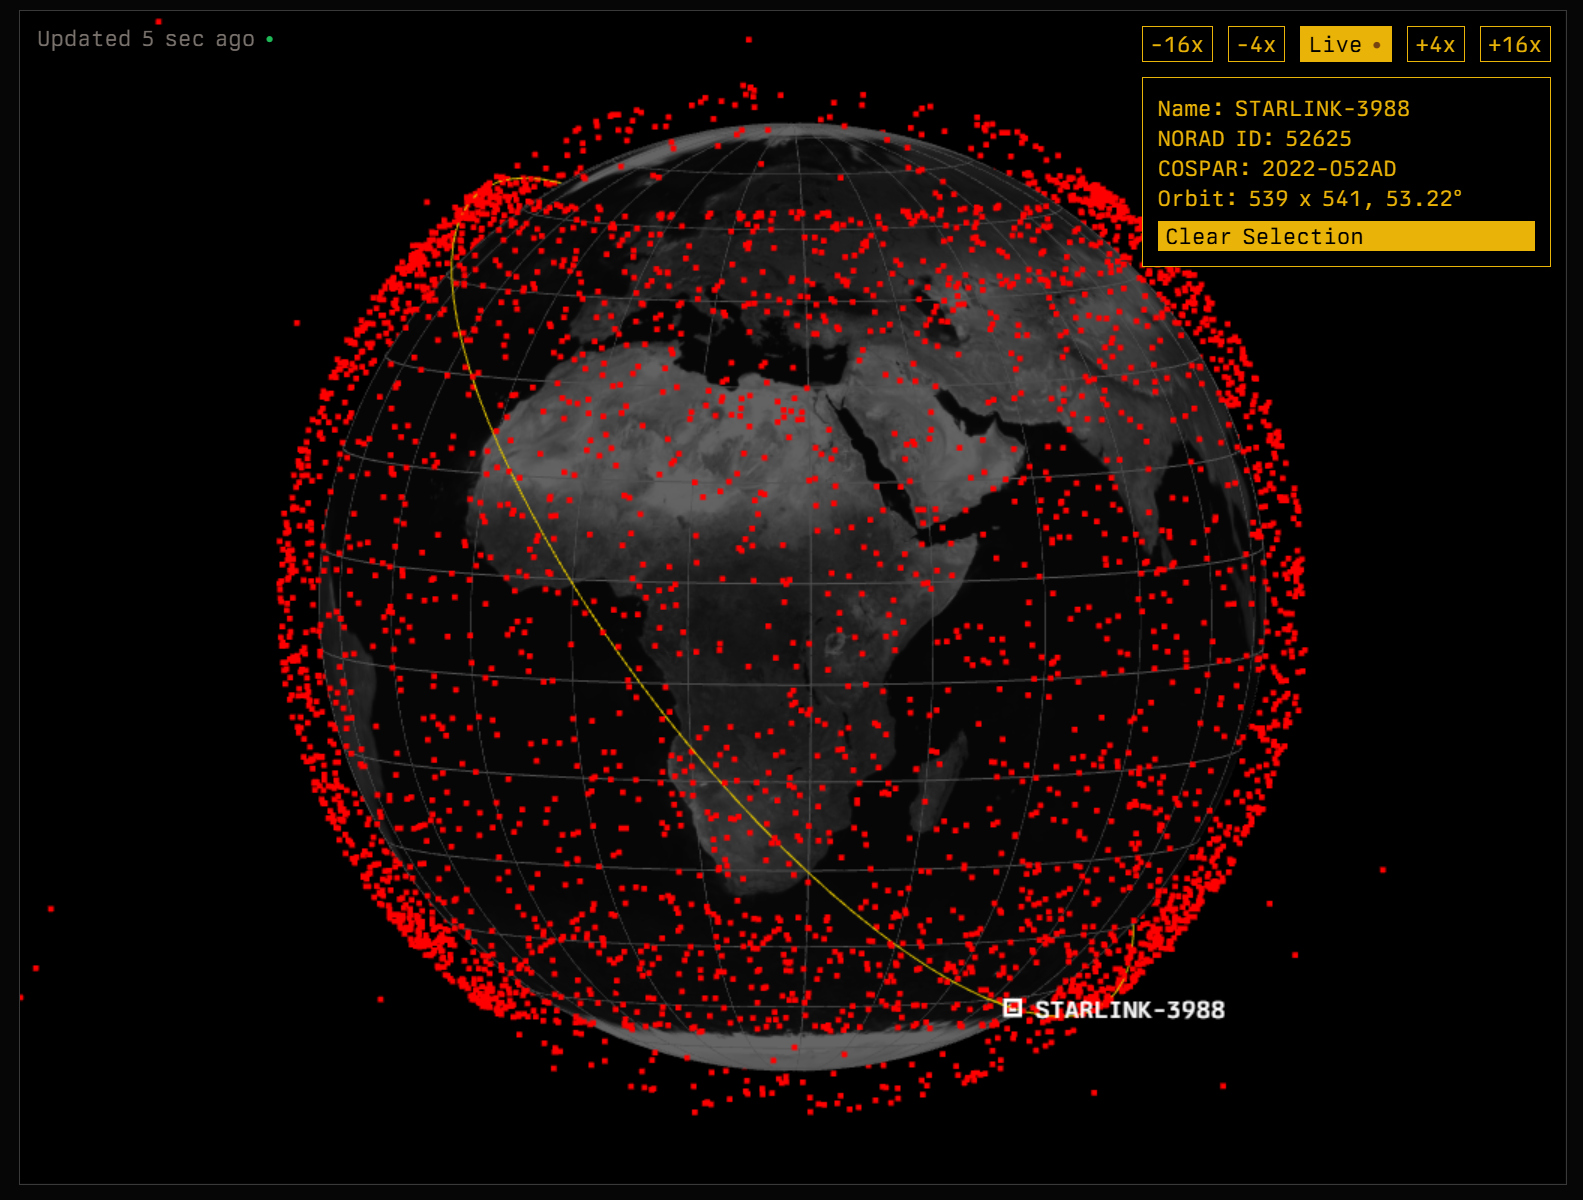
\includegraphics[width=\textwidth]{LaTeX/Figures/Starlink Constellation.png}
    \caption{Starlink constellation as of October 19th 2025, 16:59:33. Each red square represents an active satellite. Highlighted in yellow is the orbital track of selected satellite \textit{Starlink-3988}, with relevant orbital information displayed. The image is a screenshot from the Starlink Map website~\cite{starlinkmap.org}.}
    \label{fig:constellation}
\end{figure}

These satellites have already been used for several key applications, including enabling WiFi connectivity in commercial airlines and cruises, providing life-critical broadband in hurricane-ravaged coastal towns and earthquake-shaken regions, and facilitating allied command and control operations in the Russo-Ukrainian War. The constellation includes nearly 9,700 satellites (as of the writing of this report), and is visualised in Figure~\ref{fig:constellation}. Each unit is equipped with four beamforming, phased array antennas, each of which electronically steers the \SI{11.7}{\giga\hertz} collimated downlink signals in real time to a \SI{24}{\kilo\metre}-diameter ground coverage cell that can serve up to 8,000 simultaneous customers. Furthermore, the satellites communicate with one another via five on-board optical lasers at vacuum light-speed, enabling lower effective latencies between far-away cities compared to underwater cables. This is particularly relevant for applications in stock market trading, where saving a few milliseconds in latency can have a huge impact on the decision-making reactions to market fluctuations. To add to the list of groundbreaking engineering innovations that SpaceX developed for Starlink satellites, the orbital insertion procedure is entirely novel: the satellites are deployed in clusters of up to 23 units\footnote{For the larger v2 model, down from up to 60 units of the smaller v1/v1.5 model} at an altitude of roughly \SI{280}{\kilo\metre}, as shown in Figure~\ref{fig:starlink_cluster}; their orbits are then slowly raised to around \SI{550}{\kilo\metre} in two stages using Krypton gas ion thrusters\footnote{This is a more cost-efficient alternative to the customary option, Xenon gas}. This unusual manoeuvre leaves the satellites bunched up in characteristic lines before successful insertion, which can be observed from the surface of the Earth as shown in Figure~\ref{fig:starlink_line}.

\begin{figure}[h!]
    \centering

    % First subfigure (left image)
    \begin{subfigure}[b]{0.49\textwidth}
        \centering
        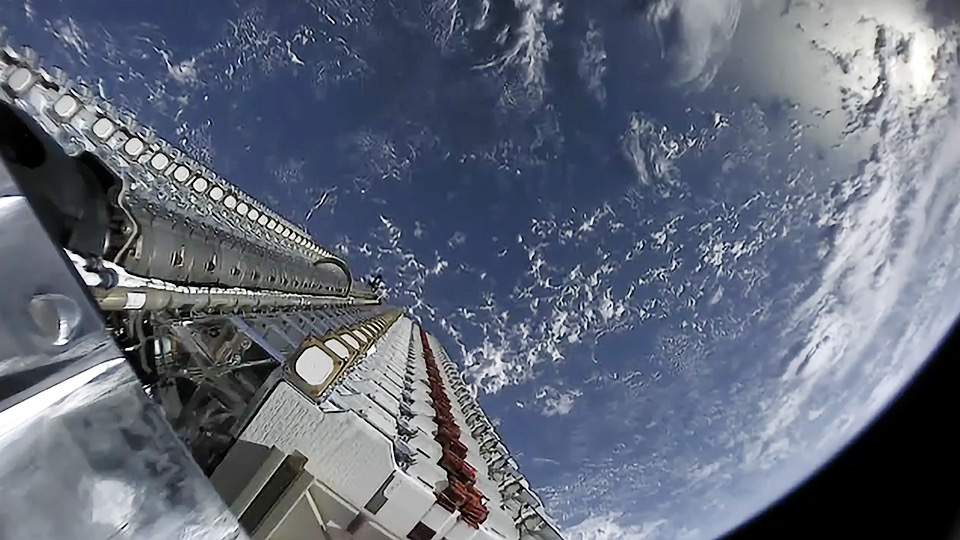
\includegraphics[width=\textwidth]{LaTeX/Figures/Starlink_cluster.jpg}
        \caption{A cluster of Starlink satellites. From~\cite{wikimedia_starlink_mission_2020}.}
        \label{fig:starlink_cluster}
    \end{subfigure}\hfill % No blank line between subfigures
    % Second subfigure (right image)
    \begin{subfigure}[b]{0.49\textwidth}
        \centering
        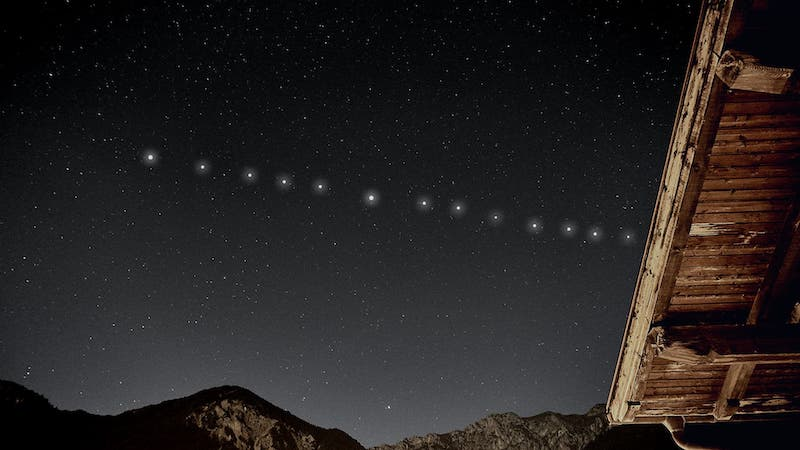
\includegraphics[width=\textwidth]{LaTeX/Figures/SPACEX-STARLINK-SATELLITES-CONSTELLATION.jpeg}
        \caption{A line of Starlink satellites. From~\cite{earthsky_starlink_2021}.}
        \label{fig:starlink_line}
    \end{subfigure}
    
\end{figure}

This project aims to investigate the orbit of an active, Earth-orbiting Starlink satellite through empirical observation and data collection. The satellite chosen is the \textit{Starlink-3988} unit, a v1.5 model as shown in Figure~\ref{fig:satellite_render}: although there aren't any attributes that distinguish it from others in the Starlink constellation, it was selected due to its favourable visibility and consistent orbital passes over Princeton, New Jersey, during the observation window (October 19–22, 2025). Furthermore, the satellite’s low-Earth orbit (LEO) characteristics, including a near-circular path, moderate inclination, and short orbital period, make it ideal for this project's requirements. A detail of the satellite's antennas is shown in Figure~\ref{fig:satellite_antennas}, and relevant attributes are reported in Table~\ref{tab:starlink3988_params}.

\begin{figure}[h!]
    \centering
    
    \begin{subfigure}[b]{0.49\textwidth}
        \centering
        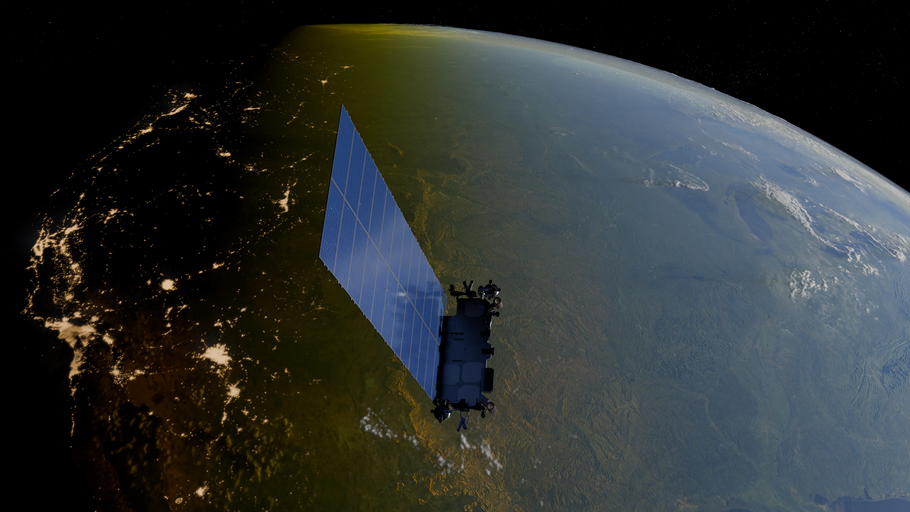
\includegraphics[width=\textwidth]{LaTeX/Figures/satellite_render.png}
        \caption{3D render of a Starlink v1.5 satellite~\cite{wikimedia_starlink_01_2025}.}
        \label{fig:satellite_render}
    \end{subfigure}\hfill
    \begin{subfigure}[b]{0.49\textwidth}
        \centering
        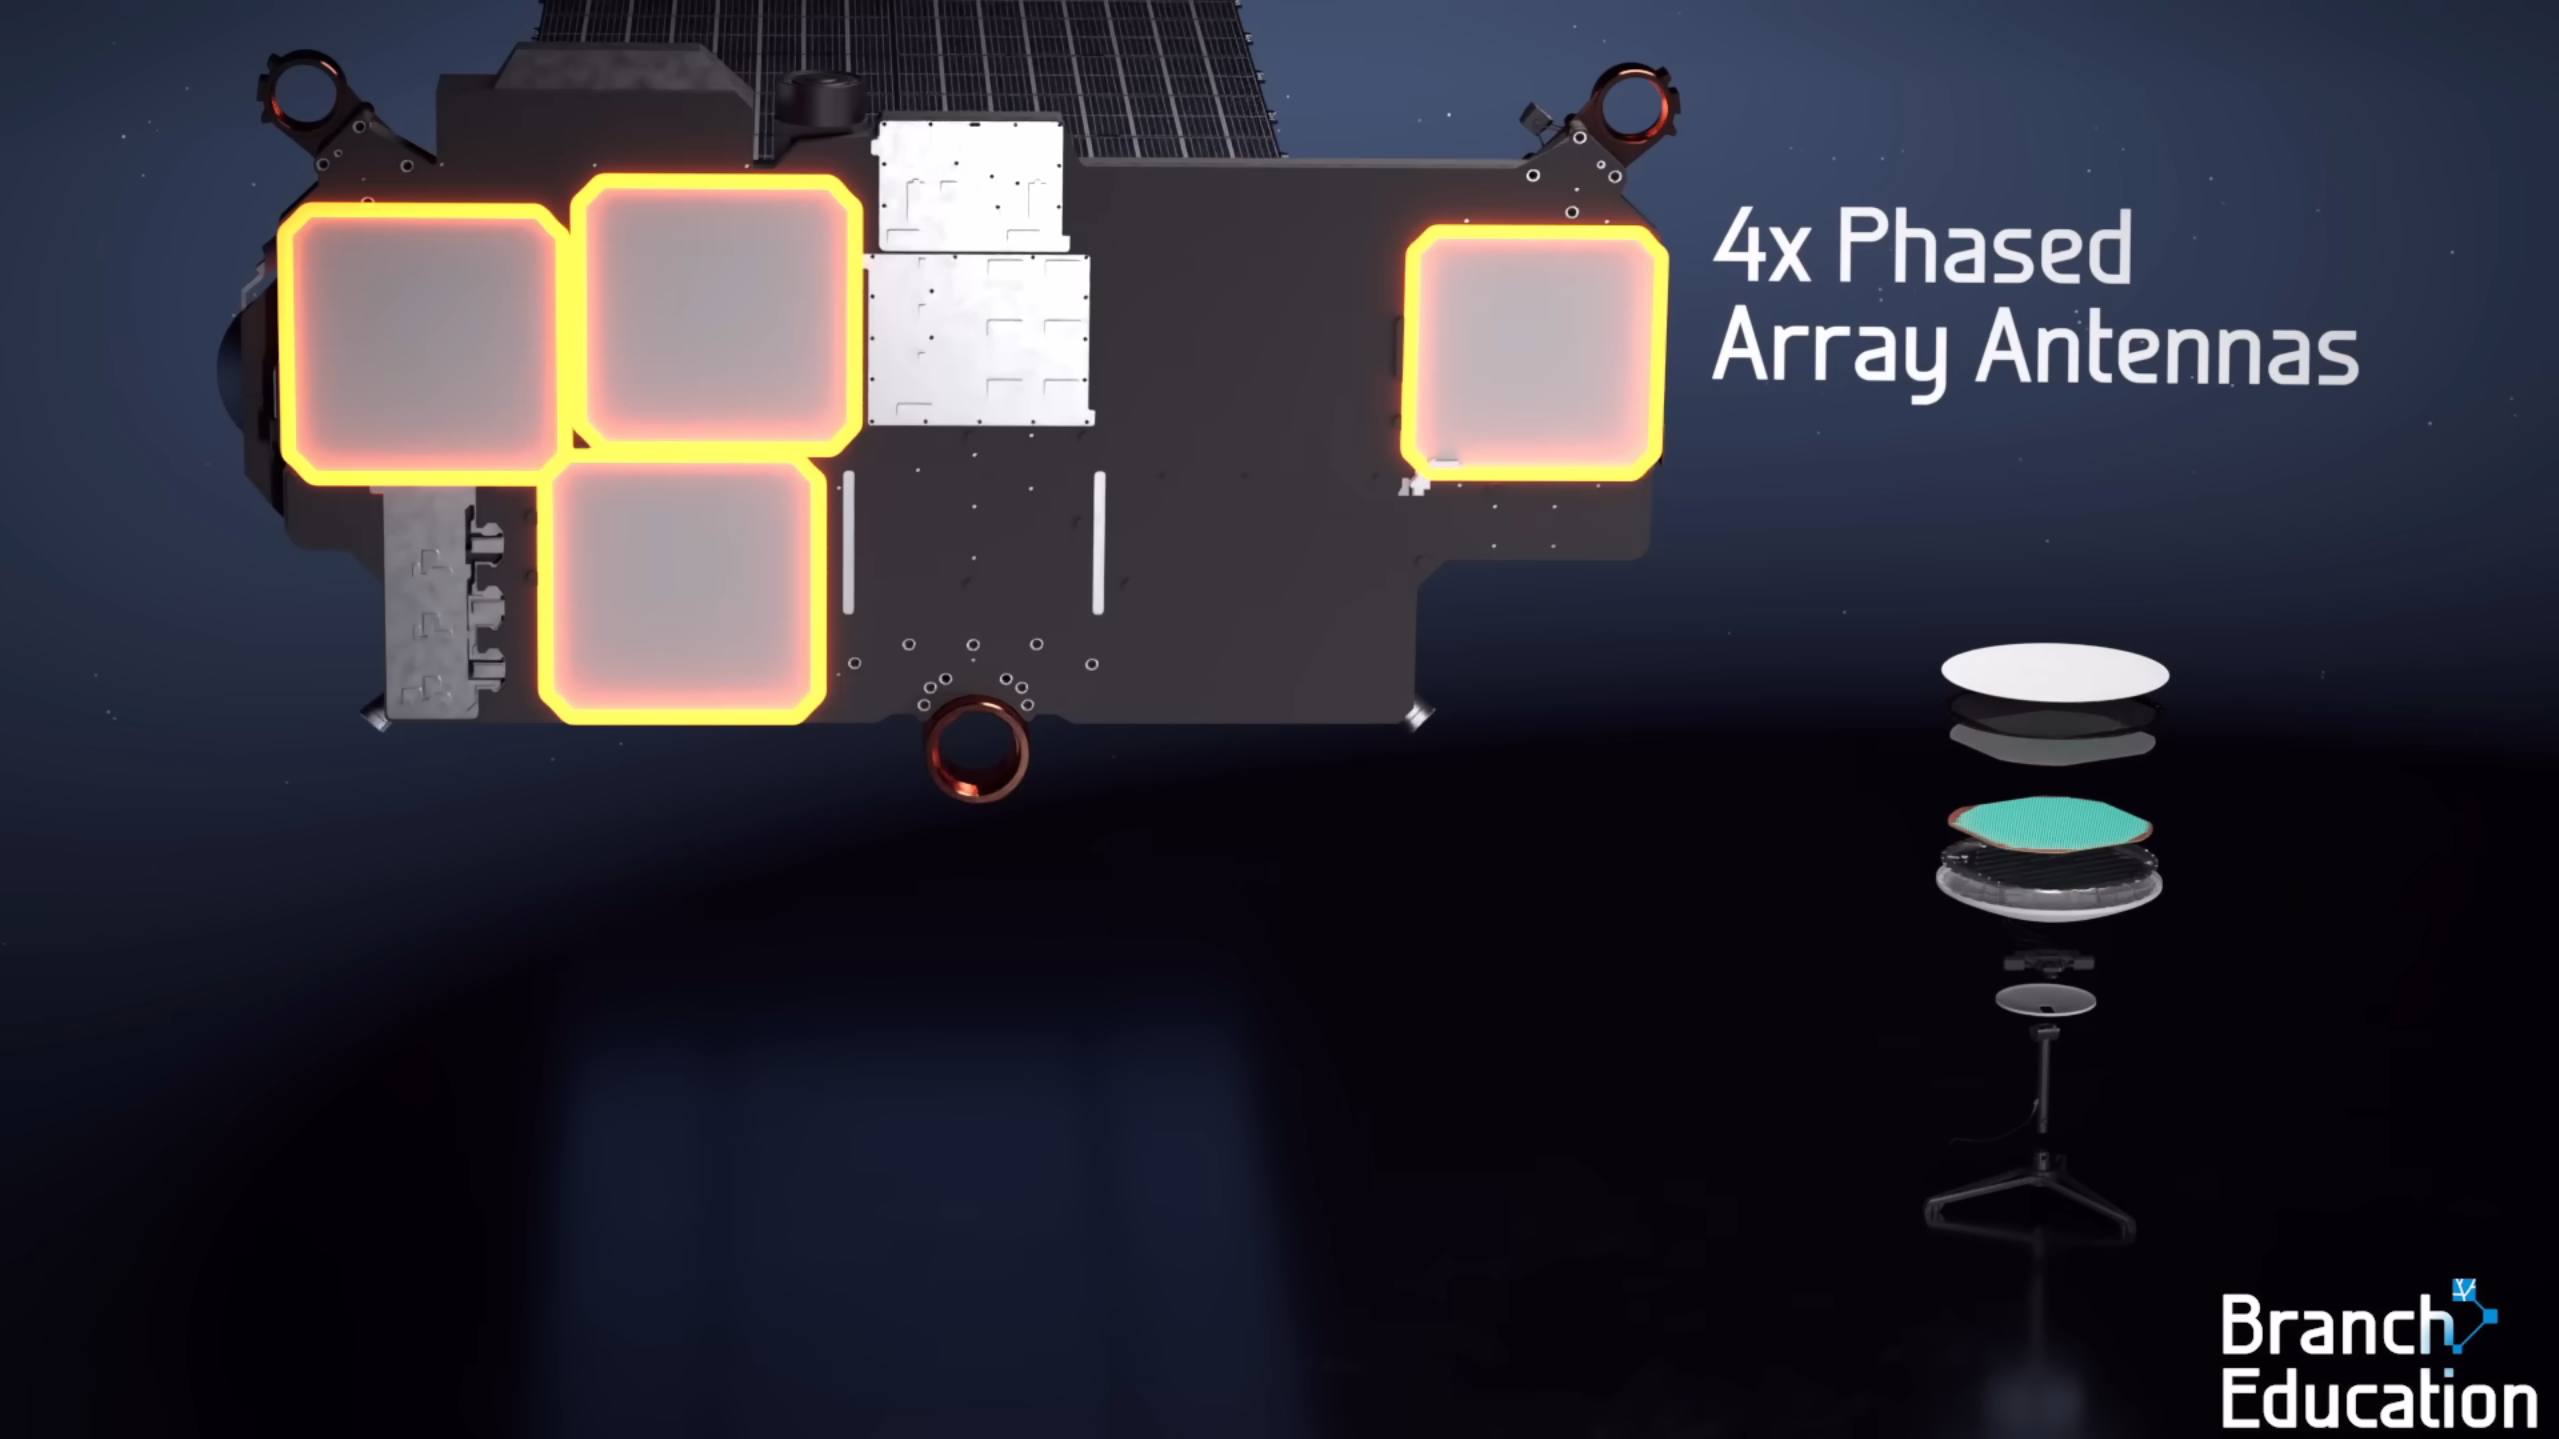
\includegraphics[width=\textwidth]{LaTeX/Figures/satellite_antennas.png}
        \caption{Satellite's antennas and dish. From~\cite{branch_education_starlink_2022}.}
        \label{fig:satellite_antennas}
    \end{subfigure}
    
\end{figure}

\begin{table}[h]
    \centering
    \caption{Identification and physical characteristics of the selected satellite \textit{Starlink-3988}. Data sourced from SpaceX public technical documentation~\cite{spacex_starlink_specs}.}
    \label{tab:starlink3988_params}
    \begin{tabular}{|l|c|}
        \hline
        \textbf{Parameter} & \textbf{Value} \\ \hline
        NORAD Catalog Number & 52625 \\ \hline
        COSPAR ID & 2022-052AD \\ \hline
        Launch Date & May 14, 2022 \\ \hline
        Launch Vehicle / Site & Falcon 9 / Cape Canaveral (AFETR) \\ \hline
        Orbit Type & Low Earth Orbit (LEO) \\ \hline
        Operational Status & Active \\ \hline
        Starlink Model & v1.5 (Laser Inter-satellite Links) \\ \hline
        Dimensions & \SI{2.8}{\metre} $\times$ \SI{1.4}{\metre} $\times$ \SI{0.2}{\metre} (without solar array) \\ \hline
        Mass & 295~\si{\kilogram} \\ \hline
    \end{tabular}
\end{table}

\newpage
\section{Data Collection} \label{sec:data}

To estimate the satellite's orbital period, two different methods were employed:

\begin{enumerate}
    \item Two overhead passes were tracked, with periodic logging of Azimuth and Elevation Angle parameters. In particular, the time of first appearance of the satellite above the horizon, followed by timestamps at every integer minute elapsed, and finally the time of disappearance of the satellite below the horizon, were all recorded. These values were then converted to Right Ascension and Declination, and, using these parameters from two distinct timestamps, the orbital period was estimated. (This corresponds to Method 1 in the instructions provided by the preceptors)
    \item The time at positions of an arbitrarily selected constant elevation angle was recorded, and the orbital period was estimated as an average of these measurements. (This corresponds to Method 4 in the instructions provided by the preceptors)
\end{enumerate}

The results from the two methods were then compared and one of the two results was selected for the remainder of the calculations.

\subsection{Method 1}

The observations of \textit{Starlink-3988} for Method 1 were performed over two separate passes above the Princeton University Art Museum, New Jersey, United States, on 19 October 2025, using a combination of qualitative and quantitative tracking techniques. The \textit{Satellite Tracker} Android application (Vito Technology) was employed for qualitative tracking of the satellite in the night sky. We first used the app to obtain a prediction of the time of appearance of the satellite above the horizon. Then, the app was used to record both the time of appearance and disappearance of the satellite above and below the horizon. On the same Android phone, time was tracked to record the precise moment each integer minute would elapse. Concurrently, the \textit{Satellite Tracker Pro} iOS application (Kornienko Vyacheslav) was used on a separate Apple phone for quantitative measurements. In coordination with time tracking from the Android phone, we logged values of Azimuth and Elevation Angles, as well as the Distance from the observer to the satellite, through consecutive screenshots. By avoiding hand logging the data in real time, the three measurements were simultaneous, and, thus, any potential transient deviation was eliminated. The operation required two mobile phones and two people (the second person involved was the author's roommate, Tomás Consonni, an Economics student who kindly provided access to his iPhone). All times were logged in Eastern Daylight Time (EDT).

The observed Azimuth and Elevation Angles, measured from the Earth's surface, were converted to Right Ascension ($\alpha$) and Declination ($\delta$). This transformation to the equatorial coordinate system, which is relative to the Earth's barycenter, was performed using a \texttt{Python} script provided by the course preceptors. We input the coordinates of our observation station as \SI{40.3463}{\degree}N, \SI{-74.6580}{\degree}E, GMT-04:00. This code also uses the distance to the satellite as an additional input. The raw data are presented in Table~\ref{tab:method1_data} below. Screenshots of the two apps for the very last measurement on the second observation (10/20 at 19:38:16) are displayed in Appendix~\ref{Appendix}.

\begin{table}[H]
    \centering
    \caption{Raw empirical data for Method 1 observations.}
    \label{tab:method1_data}
    \renewcommand{\arraystretch}{1.2}
    \begin{tabular}{|c|c|c|c|c|c|c|}
        \hline
        \textbf{Date} & \textbf{Time} & \textbf{Azimuth} & \textbf{Elevation} & \textbf{Distance} & \textbf{Right} & \textbf{Declination} \\ 
        \textbf{(2025)} & \textbf{(EDT)} & \textbf{(°)} & \textbf{Angle (°)} & \textbf{(km)} & \textbf{Ascension (°)} & \textbf{(°)} \\ \hline
        \multicolumn{7}{|c|}{\textbf{Observation 1 – 19 October 2025}} \\ \hline
        10/19 & 21:18:49 & 287.6 & 10.2 & 1628 & 315.8 & 42.8 \\ \hline
        10/19 & 21:19:00 & 286.3 & 11.0 & 1576 & 316.5 & 42.5 \\ \hline
        10/19 & 21:20:00 & 273.1 & 17.9 & 1226 & 321.0 & 39.9 \\ \hline
        10/19 & 21:21:00 & 262.7 & 21.8 & 1083 & 323.4 & 38.5 \\ \hline
        10/19 & 21:22:00 & 241.0 & 26.3 &  954 & 326.5 & 36.3 \\ \hline
        10/19 & 21:23:00 & 213.6 & 25.9 &  541 & 331.7 & 36.5 \\ \hline
        10/19 & 21:24:00 & 190.3 & 20.2 & 1137 & 333.0 & 31.2 \\ \hline
        10/19 & 21:25:00 & 176.0 & 13.7 & 1419 & 336.0 & 28.5 \\ \hline
        10/19 & 21:25:38 & 169.3 & 10.1 & 1657 & 338.0 & 26.5 \\ \hline
        \multicolumn{7}{|c|}{\textbf{Observation 2 – 20 October 2025}} \\ \hline
        10/20 & 19:31:03 & 319.7 & 10.5 & 1636 & 294.0 & 49.7 \\ \hline
        10/20 & 19:32:00 & 325.7 & 17.5 & 1264 & 299.3 & 48.2 \\ \hline
        10/20 & 19:33:00 & 337.5 & 28.0 &  930 & 304.2 & 46.4 \\ \hline
        10/20 & 19:34:00 & 006.1 & 42.2 &  694 & 308.9 & 44.4 \\ \hline
        10/20 & 19:35:00 & 056.7 & 43.7 &  677 & 313.2 & 42.2 \\ \hline
        10/20 & 19:36:00 & 088.6 & 29.9 &  886 & 317.2 & 39.9 \\ \hline
        10/20 & 19:37:00 & 101.9 & 18.6 & 1216 & 321.0 & 37.4 \\ \hline
        10/20 & 19:38:00 & 108.3 & 11.3 & 1579 & 324.4 & 34.9 \\ \hline
        10/20 & 19:38:16 & 109.5 & 09.8 & 1675 & 325.3 & 34.3 \\ \hline
    \end{tabular}
\end{table}

In preparation for the real observation, a test logging of data was also performed using the \textit{In The Sky} website. These data can be found in Appendix~\ref{Appendix} and do not contain distance to satellite entries.

\subsection{Method 4}

For the implementation of Method 4, we employed a similar experimental setup. Observations were conducted from Princeton University Art Museum, New Jersey, United States, during the 20th and 21st of October 2025.

\begin{table}[H]
    \centering
    \caption{Raw empirical data for Method 4 observations.}
    \label{tab:method4_data}
    \renewcommand{\arraystretch}{1.2}
    \begin{tabular}{|c|c|c|c|c|}
        \hline
        \textbf{Date (2025)} & \textbf{Time (EDT)} & \textbf{Elevation Angle (°)} & \textbf{Latitude (°N)} & \textbf{Longitude (°E)} \\ \hline
        \multicolumn{5}{|c|}{\textbf{Observations – 21 October 2025}} \\ \hline
        10/20 & 15:10:29 & -80.0 & -43.63 & 79.67\\ \hline
        10/20 & 16:49:20 & -80.0 & -58.24 & 72.31\\ \hline
        10/20 & 18:27:27 & -80.0 & -63.85 & 73.79\\ \hline
        10/21 & 16:59:42 & -80.0 & -48.42 & 129.85\\ \hline
        10/21 & 18:40:59 & -80.0 & -35.67 & 128.85\\ \hline
        10/21 & 20:24:44 & -80.0 & -23.76 & 116.68 \\ \hline
    \end{tabular}
\end{table}


 The \textit{N2YO} website (\href{https://www.n2yo.com}{https://www.n2yo.com}) was employed for quantitative tracking: we screen-recorded a portion of the website containing data about time, Elevation Angle, latitude and longitude over several hours of time on two separate days. The recorded footage was later analysed to extract precise timestamps at which the satellite crossed a constant elevation angle during each pass. By employing this technique, a consistent dataset was obtained without the need for manual data entry, thereby reducing human timing errors. An example screenshot of the data obtained from the screen recording is displayed in Appendix~\ref{Appendix}. All times were recorded in Eastern Daylight Time (EDT). The elapsed times between consecutive passes at the same elevation will be used to estimate the orbital period. The raw data are summarised in Table~\ref{tab:method4_data}.

\section{Estimate of Period and Angular Velocity} \label{first_estimates_and_assumptions}

The purpose of this section is to calculate orbital period and angular velocity for the \textit{Starlink-3988} satellite using the data presented in Section~\ref{sec:data}. All calculations were performed using \texttt{Python}, and scripts can be found at the supporting repository:
\begin{center}
    \href{https://github.com/ClouD-161803/MAE341-Project1}{ClouD-161803/MAE341-Project1}.
\end{center}

To carry out the calculations below, we made several simplifying assumptions:

\begin{itemize}
    \item The mass of the satellite is negligible when compared to that of the Earth, so the Earth remains stationary whilst the satellite is orbiting it.
    \item The orbital influence of any perturbations to the two-body problem, including gravitational field distortions due to Earth's shape, atmospheric drag, lunisolar perturbations, and solar radiation pressure, was assumed to be negligible and was not accounted for in our methods.
    \item For processing data emanating from Method 1 collection, we assumed the orbital path traced by the satellite is a perfect circle. This assumption implies that the true anomaly and the eccentric anomaly are equal at all times. We will show the validity of this assumption when evaluating the (elliptical) orbit's eccentricity, and show that it is very close to the assumed value of $0$. As a result, the satellite is assumed to be travelling in a straight line on the surface of a 2-sphere (whose radius is the orbital radius, i.e. Earth's radius plus altitude). This path is also known as a geodesic.
    \item For processing data emanating from Method 4 collection, we assumed that the satellite completes a full orbit when crossing the same elevation angle at two separate times. Note that the condition to be met is that both the elevation angle's value \emph{and} the sign of its rate of change (positive for ascension, negative for descent) are equal. It is noted that, within each orbit, the satellite passes a given elevation angle \emph{twice}, once on ascent and once on descent. We were careful to consider the descent timestep for each orbital pass. 
\end{itemize}

The following constants were used throughout for numerical evaluation of all parameters:

\begin{center}
    \vspace{0.5em}
    
    \begin{tabular}{l c}
        Earth gravitational parameter & $\mu_{\text{E}} = \SI{398574}{\kilo\meter^3\per\second^2}$ \\[0.3em]
        Mean radius of Earth & $R_{\text{E}} = \SI{6378}{\kilo\meter}$ \\[0.3em]
        Mass of Earth & $M_{\text{E}} = \SI{5.9722e24}{\kilogram}$ \\[0.3em]
    \end{tabular}
\end{center}

\subsection{Orbital Period}

\subsubsection{Method 4}

Using Method~4, the orbital period is determined from the elapsed time between successive appearances of the satellite at a fixed elevation angle. Our selection of angle fell on an elevation angle of $-80^{\circ}$ (for no particular reason). By computing the time interval between successive passes of identical elevation, the orbital period $\tau$ can be estimated directly as the difference in observation times. The resulting orbital periods for each consecutive pass are presented in Table~\ref{tab:method4_periods}. The intervals were converted to minutes and compared with the published value ($\tau_{\text{true}} = \SI{95.4}{\minute}$).

\begin{table}[H]
    \centering
    \caption{Orbital period estimates using Method~4 (constant elevation angle).}
    \label{tab:method4_periods}
    \renewcommand{\arraystretch}{1.2}
    \begin{tabular}{|c|c|c|c|}
        \hline
        \textbf{Pass Interval} & \textbf{Time Difference (hh:mm:ss)} & \textbf{$\tau$ (\si{\minute})} & \textbf{Error vs. True (\%)} \\ \hline
        1–2 & 01:38:51 & 98.85 & +3.61 \\ \hline
        2–3 & 01:38:07 & 98.12 & +2.84 \\ \hline
        4–5 & 01:41:17 & 101.28 & +6.15 \\ \hline
        5–6 & 01:43:45 & 103.75 & +8.73 \\ \hline
        \textbf{Mean} &  & \textbf{100.00} & \textbf{+4.81} \\ \hline
    \end{tabular}
\end{table}

From Table~\ref{tab:method4_periods}, the mean orbital period obtained via Method~4 was $\bar{\tau}_{4} = \SI{100.0}{\minute}$, which exceeds the true period by approximately \SI{4.8}{\percent}. This systematic overestimation likely stems from the relatively coarse time resolution of the available constant-elevation data and potential timing offsets in the dataset. Moreover, Method~4 is sensitive to local geometric distortions in elevation tracking and assumes perfectly consistent ground geometry between passes, which is likely not achieved in practice as the satellite's position above the Earth changes with each orbit (notice the drift in Latitude and Longitude from Table~\ref{tab:method4_data}). Therefore, although Method~4 provides a reasonable first-order estimate, its reliance on single-point elevation measurements introduces significant temporal and geometric uncertainty. The method is simple to apply when constant-elevation crossings are clearly recorded, but it is be vulnerable to several sources of error.

\subsubsection{Method 1}

Using Method 1, we calculated several pairs of Right Ascension ($\alpha$) and Declination ($\delta$) coordinates. The selected data points for the calculations following correspond to the Second Observation half of Table~\ref{tab:method1_data}. For two consecutive observations of the satellite separated by a known time interval $\Delta t$, the angular displacement $\psi$ on the celestial sphere is approximated using the arc of geodesic separating the two points:

\[
    \cos{\psi} = \sin{\delta_1}\sin{\delta_2} + \cos{\delta_1}\cos{\delta_2}\cos{(\alpha_2 - \alpha_1)}.
    \label{eq:psi_equation}
\]

The corresponding angular distance $\psi$ (in radians) is then:

\begin{equation}
    \psi = \cos^{-1}\!\left[\sin{\delta_1}\sin{\delta_2} + \cos{\delta_1}\cos{\delta_2}\cos{(\alpha_2 - \alpha_1)}\right].
    \label{eq:psi_angle}
\end{equation}

For a circular orbit, the orbital period $\tau$ can be estimated from the total angular displacement of $2\pi$ radians over one revolution, rearranging the relation between $\psi$, $\Delta t$, and $\tau$ as follows:

\begin{equation}
    \tau = \frac{2\pi\,\Delta t}{\psi}.
    \label{eq:tau_from_psi}
\end{equation}

Several pairs of observations were selected from the Second Observation session of Table~\ref{tab:method1_data} (10/20/2025) to evaluate the consistency of the result. The values of $\psi$, angular velocity $\omega$ were computed in a parallel fashion using~\eqref{eq:psi_angle}, and the resulting period $\tau$ with~\eqref{eq:tau_from_psi}. The results are summarised in Table~\ref{tab:psi_periods}, and plotted in Figure~\ref{fig:psi_periods_plot}.

\begin{table}[H]
    \centering
    \caption{Orbital period estimates using Method~1 for various right ascension/declination pairs from Observation 2 (10/20) of Method 1.}
    \label{tab:psi_periods}
    \renewcommand{\arraystretch}{1.15}
    \begin{tabular}{|c|c|c|c|c|}
        \hline
        \textbf{Pair} & $\Delta t$ (\si{\second}) & $\psi$ (\si{\degree}) & $\omega$ (\si{\degree\per\second}) & $\tau$ (\si{\minute}) \\ \hline
        1--5 & 237 & 15.2228 & 0.064231 & 93.41 \\ \hline
        2--6 & 240 & 15.2429 & 0.063512 & 94.47 \\ \hline
        3--7 & 240 & 15.2914 & 0.063714 & 94.17 \\ \hline
        4--8 & 240 & 15.1641 & 0.063184 & 94.96 \\ \hline
        1--6 & 297 & 19.0336 & 0.064086 & 93.62 \\ \hline
        2--7 & 300 & 19.1123 & 0.063708 & 94.18 \\ \hline
        3--8 & 300 & 19.0354 & 0.063451 & 94.56 \\ \hline
        1--7 & 357 & 22.9031 & 0.064154 & 93.53 \\ \hline
        2--8 & 360 & 22.8563 & 0.063490 & 94.50 \\ \hline
        1--8 & 417 & 26.6471 & 0.063902 & 93.89 \\ \hline
    \end{tabular}
\end{table}

From the ten independent estimates in Table~\ref{tab:psi_periods}, the mean period and standard deviation were computed as:
\[
\bar{\tau} = \SI{94.13}{\minute}, \qquad \sigma_\tau = \SI{0.50}{\minute}.
\]
These results exhibit strong consistency across all selected pairs, with less than \SI{1}{\minute} of spread.  
The small scatter reflects good internal precision but does not include potential systematic uncertainties, such as timing offsets, coordinate conversion accuracy, or deviations from the circular orbit assumption.

\begin{figure}[H]
    \centering
    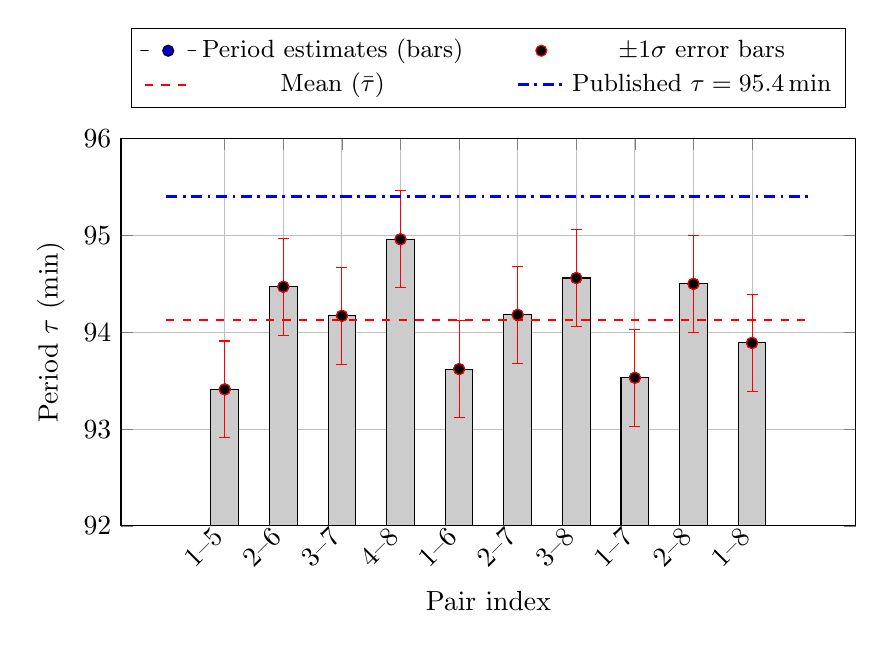
\begin{tikzpicture}
        \begin{axis}[
            width=0.9\linewidth,
            height=6.5cm,
            xlabel={Pair index},
            ylabel={Period $\tau$ (\si{\minute})},
            ymin=92, ymax=96,
            xtick={1,...,10},
            xticklabels={1--5,2--6,3--7,4--8,1--6,2--7,3--8,1--7,2--8,1--8},
            x tick label style={rotate=45, anchor=east},
            grid=major,
            bar width=10pt,
            enlarge x limits=0.07,
            legend style={
                at={(0.5,1.08)},
                anchor=south,
                draw=black,
                fill=white,
                font=\small,
                legend columns=2,
                /tikz/every even column/.append style={column sep=0.6cm}
            }
        ]
        % Bar chart of the period estimates
        \addplot+[ybar, fill=gray!40, draw=black] coordinates {
            (1,93.41) (2,94.47) (3,94.17) (4,94.96) (5,93.62)
            (6,94.18) (7,94.56) (8,93.53) (9,94.50) (10,93.89)
        };
        % Error bars (±1 sigma) as black markers with error bars
        \addplot+[only marks, mark=*, mark options={fill=black}, error bars/.cd, y dir=both, y explicit]
        coordinates {
            (1,93.41) +- (0,0.50)
            (2,94.47) +- (0,0.50)
            (3,94.17) +- (0,0.50)
            (4,94.96) +- (0,0.50)
            (5,93.62) +- (0,0.50)
            (6,94.18) +- (0,0.50)
            (7,94.56) +- (0,0.50)
            (8,93.53) +- (0,0.50)
            (9,94.50) +- (0,0.50)
            (10,93.89) +- (0,0.50)
        };
        % Mean line (dashed red)
        \addplot [red, thick, dashed] coordinates {(0,94.13) (11,94.13)};
        % Published / stated value line (dot-dashed blue)
        \addplot [blue, very thick, dash pattern=on 4pt off 2pt on 1pt off 2pt] coordinates {(0,95.40) (11,95.40)};
        % Legend (two columns, two rows)
        \legend{
            Period estimates (bars),
            $\pm1\sigma$ error bars,
            Mean ($\bar{\tau}$),
            Published $\tau=95.4\,$min
        }
        \end{axis}
    \end{tikzpicture}
    \caption{Orbital period estimates for each observation pair: bars show individual estimates, black markers with error bars indicate $\pm1\sigma$ uncertainty, the dashed red line represents the mean estimate ($\bar{\tau}=\SI{94.13}{\minute}$), and the blue dot-dashed line marks the published value ($\tau=\SI{95.4}{\minute}$).}
    \label{fig:psi_periods_plot}
\end{figure}

Taking the mean value $\bar{\tau} = \SI{94.13}{\minute}$ as the best estimate for the orbital period and comparing it with the published value of \SI{95.4}{\minute}~\cite{n2yo_starlink3988}, the percentage error is
\[
\varepsilon = \frac{|\bar{\tau} - \tau_\text{true}|}{\tau_\text{true}} \times 100
           = \frac{|94.13 - 95.4|}{95.4} \times 100 = \SI{1.33}{\percent}.
\]

We noted that all of the measurements involving index~1 were systematically below the empirical mean value, often outside of the $1\sigma$ range. This points to a likely human error in the measurement of the first timestamp for the second observation. To refine the estimate, we removed all pairs containing index~1 from the dataset and recomputed the mean and standard deviation, plotting the results in Figure~\ref{fig:psi_periods_refined}. The recalculated statistics were:
\[
\bar{\tau}_{\text{refined}} = \SI{94.47}{\minute}, \qquad \sigma_{\tau,\text{refined}} = \SI{0.46}{\minute}.
\]

\subsubsection{Comparison}

Method~4 produced a mean $\bar{\tau}_{4}=\SI{100.0}{\minute}$ (error vs.\ published value of +\SI{4.8}{\percent}), whereas the refined Method~1 result is $\bar{\tau}_{\text{refined}}=\SI{94.47}{\minute}$ (error vs.\ published value of \SI{0.97}{\percent}). Method~1 therefore yields both a closer agreement with the published orbital period and a much smaller internal scatter (after removing the identified systematic involving index~1). Method~4 is straightforward to apply when constant-elevation events are reliably recorded, but it is more vulnerable to timing bias, mis-identification of passes, and projection/geometric effects. Method~1 requires more processing (coordinate transformations and pairwise angular calculations) but benefits from averaging many angular separations on the celestial sphere and is less sensitive to a single erroneous timestamp, and hence is more reliable. Therefore, we chose the results of Method 1.

\begin{figure}[h]
    \centering
    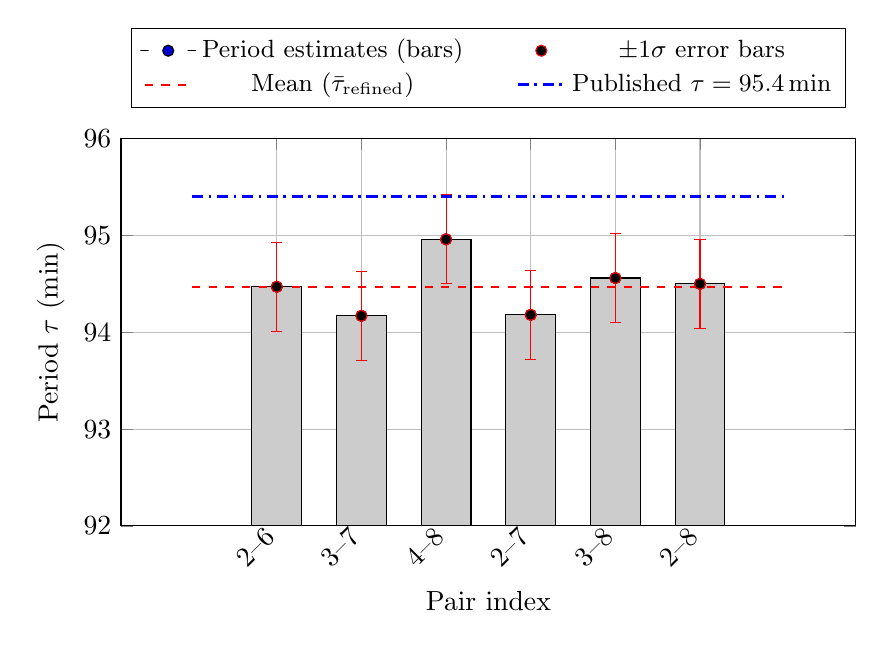
\begin{tikzpicture}
        \begin{axis}[
            width=0.9\linewidth,
            height=6.5cm,
            xlabel={Pair index},
            ylabel={Period $\tau$ (\si{\minute})},
            ymin=92, ymax=96,
            xtick={1,...,6},
            xticklabels={2--6,3--7,4--8,2--7,3--8,2--8},
            x tick label style={rotate=45, anchor=east},
            grid=major,
            bar width=18pt,
            enlarge x limits=0.12,
            legend style={
                at={(0.5,1.08)},
                anchor=south,
                draw=black,
                fill=white,
                font=\small,
                legend columns=2,
                /tikz/every even column/.append style={column sep=0.6cm}
            }
        ]
        % Bar chart of the refined period estimates (pairs without index 1)
        \addplot+[ybar, fill=gray!40, draw=black] coordinates {
            (1,94.47) (2,94.17) (3,94.96) (4,94.18) (5,94.56) (6,94.50)
        };
        % Error bars (±1 sigma, refined) as black markers with error bars, superimposed
        \addplot+[only marks, mark=*, mark options={fill=black}, error bars/.cd, y dir=both, y explicit]
        coordinates {
            (1,94.47) +- (0,0.46)
            (2,94.17) +- (0,0.46)
            (3,94.96) +- (0,0.46)
            (4,94.18) +- (0,0.46)
            (5,94.56) +- (0,0.46)
            (6,94.50) +- (0,0.46)
        };
        % Refined mean line (dashed red)
        \addplot [red, thick, dashed] coordinates {(0,94.47) (7,94.47)};
        % Published / stated value line (dot-dashed blue)
        \addplot [blue, very thick, dash pattern=on 4pt off 2pt on 1pt off 2pt] coordinates {(0,95.40) (7,95.40)};
        % Legend (two columns)
        \legend{
            Period estimates (bars),
            $\pm1\sigma$ error bars,
            Mean ($\bar{\tau}_{\mathrm{refined}}$),
            Published $\tau=95.4\,$min
        }
        \end{axis}
    \end{tikzpicture}
    \caption{Refined orbital period estimates (pairs excluding index~1). Bars show individual estimates, black markers with error bars indicate $\pm1\sigma$ uncertainty (using the refined $\sigma_{\tau}=\SI{0.46}{\minute}$), the dashed red line represents the refined mean ($\bar{\tau}_{\mathrm{refined}}=\SI{94.47}{\minute}$), and the blue dot-dashed line marks the published value ($\tau=\SI{95.4}{\minute}$).}
    \label{fig:psi_periods_refined}
\end{figure}

\subsection{Angular Velocity}

Keeping index~1 excluded from the dataset, we also computed the corresponding mean angular velocity, defined as \[ \omega = \frac{2\pi}{\tau}. \] Using the refined mean orbital period $\bar{\tau}_{\text{refined}} = \SI{94.47}{\minute}$, the resulting mean angular velocity is \[ \bar{\omega}_{\text{refined}} = \frac{2\pi}{94.47\times60} = \SI{0.001108}{\radian\per\second} = \SI{0.06347}{\degree\per\second}. \] The uncertainty in $\omega$ measurement arises from the propagation of the period uncertainty, $\sigma_{\tau,\text{refined}} = \SI{0.46}{\minute}$, through the inverse relationship $\omega \propto 1/\tau$, and is also very small, indicating internal consistency.

We adopt the refined values from Method~1:
\[
    \boxed{
    \bar{\tau}_{\text{refined}} = \SI{94.47}{\minute}, \qquad 
    \bar{\omega}_{\text{refined}} = \SI{1.108e-3}{\radian\per\second}}
\]
as the definitive parameters for all subsequent orbital calculations in this report.

\section{Estimate of Semi-Major Axis and Position Prediction}

The remainder of this report is concerned with the evaluation of orbital elements for the orbit of the \textit{Starlink-3988} satellite. In general, orbital elements are a set of parameters that fully define the shape of a satellite's orbit around a central body, as well as the position of the satellite along the orbit, effectively nailing the location of the satellite in 3D space at a given time relative to a given reference frame. The most common set of orbital parameters to describe orbits of satellites around the Earth is that of the six orbital elements: eccentricity ($e$), semi-major axis ($a$), inclination ($i$), longitude (right ascension) of the ascending node ($\Omega$), argument of periapsis ($\omega$), and true anomaly ($\theta$). For reference and comparison, the ground truth TLE values for the \textit{Starlink-3988} satellite are given in Table~\ref{tab:starlink3988_orbit}. These were taken from the \textit{N2YO} website, and a full explanation of how we converted the raw TLEs to the values in the table is given in Appendix~\ref{AppendixB}. In this section, we will evaluate the semi-major axis, and carry out a point prediction of the position of the satellite in the future, and compare our results to the ground truth values from Table~\ref{tab:starlink3988_orbit}.

\begin{table}[h]
    \centering
    \caption{Orbital parameters for \textit{Starlink-3988}. Data sourced from N2YO~\cite{n2yo_starlink3988} at 18:53:19~EDT.}
    \label{tab:starlink3988_orbit}
    \begin{tabular}{|l|c|c|}
        \hline
        \textbf{Parameter} & \textbf{Symbol / Unit} & \textbf{TLE Value} \\ \hline
        Date & $(YYYY-MM-DD)$ & 2025-10-21 \\ \hline
        Epoch (UTC) & $(hh:mm:ss)$ & 22:53:19 \\ \hline
        Inclination & $i$ (\si{\degree}) & 53.2146 \\ \hline
        Right Ascension of Ascending Node & $\Omega$ (\si{\degree}) & 171.9324 \\ \hline
        Eccentricity & $e$ () & 0.0001133 \\ \hline
        Argument of Perigee & $\omega$ (\si{\degree}) & 95.0058 \\ \hline
        Semi-Major Axis & $a$ (\si{\kilo\metre}) & 6917 \\ \hline
        Mean Anomaly & $M$ (\si{\degree}) & 265.1064 \\ \hline
        Perigee Altitude & $h_p$ (\si{\kilo\metre}) & 545.9 \\ \hline
        Apogee Altitude & $h_a$ (\si{\kilo\metre}) & 547.9 \\ \hline
        Mean Altitude & $h$ (\si{\kilo\metre}) & 546.9 \\ \hline
        Orbital Period & $\tau$ (\si{\minute}) & 95.43 \\ \hline
        Mean Motion & $n$ (\si{rev/day}) & 15.088489 \\ \hline
    \end{tabular}
\end{table}

\subsection{Semi-Major Axis}

The semi-major axis of a satellite's closed elliptical orbit refers to half the distance that separates the point of closest approach to the centre of the Earth (perigee) to that of furthest distance away (apogee). Naturally, it has dimensions of length. From Kepler's third law, the semi-major axis is related to the orbital period via:

\[
\tau^{2} = \frac{4\pi^{2}}{\mu} a^{3},
\]
where $\mu$ is Earth's standard gravitational parameter.  
Rearranging for $a$ gives:
\begin{equation}
\label{semi_major_axis_from_tau}
    a = \left( \frac{\mu \tau^{2}}{4\pi^{2}} \right)^{1/3}.
\end{equation}

Using the refined orbital period obtained previously of $\bar{\tau} = \SI{94.47}{\minute}$, which corresponds to:
\[
\bar{\tau} = \SI{94.47}{\minute} \times \SI{60}{\second\per\minute} = \SI{5668}{\second},
\]
we substitute into~\eqref{semi_major_axis_from_tau}:
\[
\bar{a} = \left( \frac{(\SI{398574}{\kilo\metre^{3}\per\second^{2}}) (\num{3.215e7})}{\num{39.478}} \right)^{1/3}
   = \left( \num{3.246e11} \right)^{1/3}.
\]
Hence:
\[
\boxed{\bar{a} = \SI{6938}{\kilo\metre}},
\]
to four significant figures.

Since the orbit was assumed to be circular (we will show this is a good assumption in Section~\ref{sec:orbital_elements}), the computed semi-major axis of $\bar{a} = \SI{6938}{\kilo\metre}$ also corresponds to the mean orbital radius of the satellite.  
For comparison, the semi-major axis derived from the satellite’s published orbital elements (Two-Line Element set, TLE) given in Table~\ref{tab:starlink3988_orbit} is:
\[
a_{\text{TLE}} = \SI{6917}{\kilo\metre}.
\]
The difference between the observed and tabulated values is therefore:
\[
\Delta a = \bar{a} - a_{\text{TLE}} = \SI{21}{\kilo\metre},
\]
corresponding to a relative error of:
\[
\frac{|\Delta a|}{a_{\text{TLE}}} \times 100 = \SI{0.30}{\percent}.
\]
This small deviation is well within experimental uncertainty and primarily arises from limited precision in the timing of orbital passes, as well as the simplifying assumption of a perfectly circular orbit ($e \approx 0$), which neglects the satellite’s small but nonzero eccentricity.

\subsection{Position Prediction via Kepler’s Equation} \label{sec:mean_anomaly}

Having determined the orbital period $\tau$ and semi-major axis $a$, we can predict the satellite’s position along its orbit at any future time using Kepler’s equation:
\begin{equation}
    \label{eq:kepler_equation}
    M_e = \varepsilon_e - e\sin \varepsilon_e,
\end{equation}
where $M_e$ is the elliptical mean anomaly and $\varepsilon_e$ is the elliptical eccentric anomaly. For small eccentricities this relation simplifies to $M_e \approx \varepsilon_e \approx \theta$, where $\theta$ denotes the true anomaly. Choosing a reference time $t_0$ corresponding to a known satellite position, the mean anomaly at a later time $t$ is given by:
\[
M_e(t) = \frac{2\pi}{\tau}(t - t_0).
\]
Substituting $M_e$ into~\eqref{eq:kepler_equation} requires an iterative solution for $\varepsilon_e$ (examples of numerical schemes are bisection or Newton's method). The radius vector is then:
\[
r = a(1 - e\cos \varepsilon_e),
\]
and the true anomaly may be recovered from the geometry of the ellipse. For circular orbits ($e \approx 0$) the computation simplifies significantly:
\[
\theta(t) = M_e(t) = \frac{2\pi}{\tau}(t - t_0).
\]
This allows direct prediction of the satellite’s angular position and corresponding ground track as a function of elapsed time. To evaluate a point prediction, we therefore need a starting time, with known value of mean anomaly, and a prediction window $t - t_0$ to evaluate against. 

\begin{figure}[h]
    \centering
    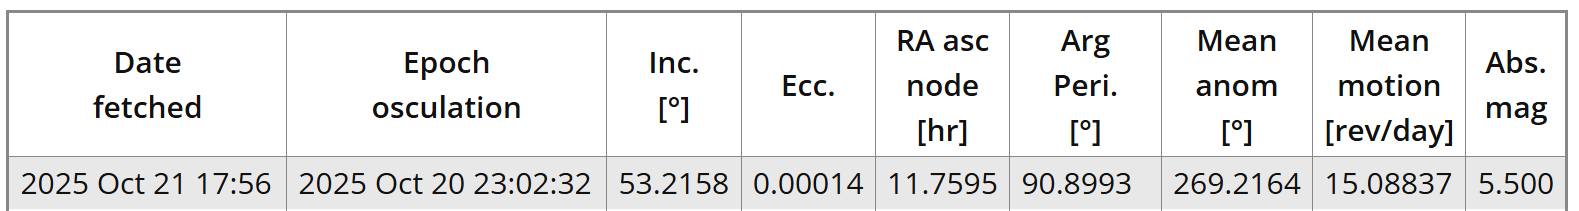
\includegraphics[width=\textwidth]{LaTeX/Figures/TLE_from_in_the_sky.png}
    \caption{Screenshot of the \textit{Starlink-3988} TLE as fetched from the \textit{In-The-Sky} website.}
    \label{fig:inthesky_tle}
\end{figure}

The choice of initial time was dictated by the availability of TLEs from online sources. The closest TLE we could obtain to our measurement timestamps was for 2025-10-20 at 23:02:32 UTC, which is very close to the measurement on the first row of Observation 2 in Table~\ref{tab:method1_data} (2025-10-20 at 19:31:03 EDT or 23:31:03 UTC, i.e. 28 minutes and 31 seconds before the satellite rose over the horizon at our location). This TLE was obtained from the \textit{In-The-Sky} website, a screenshot of which is given in Figure~\ref{fig:inthesky_tle}. The mean anomaly reported at this osculation epoch is \(M_{0}=\SI{269.2164}{\degree}\). The target time is that of the TLE of Table~\ref{tab:starlink3988_orbit}, namely \(t=\) 2025-10-21 18:53:19 EDT \(=\) 2025-10-21 22:53:19 UTC. The elapsed time is therefore:
\[
\Delta t = t - t_{0}
= \text{2025-10-21 22:53:19 UTC} - \text{2025-10-20 23:02:32 UTC}
= \SI{85847}{\second}.
\]
Using the observational estimate \(\bar{\tau}=\SI{94.47}{\minute}=\SI{5668.2}{\second}\) to propagate mean anomaly forward, the number of revolutions during \(\Delta t\) is:
\[
\Delta N = \frac{\Delta t}{\bar{\tau}}
= \frac{\SI{85847}{\second}}{\SI{5668.2}{\second}}
= \num{15.14537243}\ \text{revolutions},
\]
which corresponds to an angular advance of:
\[
\Delta M = 360^\circ\,\Delta N
= 360^\circ\times\num{15.14537243}
= \SI{5452.3341}{\degree}.
\]
Adding this advance to the initial mean anomaly gives:
\[
\bar{M}_{e} = M_{0} + \Delta M
= \SI{269.2164}{\degree} + \SI{5452.3341}{\degree}
= \SI{5721.5505}{\degree}.
\]
Reduced to the principal range \([0^\circ,360^\circ)\), using a modulo 360 operation, this becomes:
\[
\boxed{\,\bar{M}_{e} = \SI{321.5505}{\degree} \;=\; \SI{5.6121}{\radian}\}}
\]
The mean anomaly reported in Table~\ref{tab:starlink3988_orbit} (the TLE value at the target epoch) is:
\[
M_{\text{TLE}} = \SI{265.1064}{\degree}.
\]
The absolute angular difference between the propagated value and the table value is:
\[
\Delta M_e = |\bar{M}_{e} - M_{\text{TLE}}| = \SI{56.4441}{\degree},
\]
which corresponds to a relative error of:
\[
\frac{\Delta M_e}{M_{\text{TLE}}}\times 100 \approx \SI{21.29}{\percent}.
\]

This percentage error is almost two orders of magnitude higher than the error on the orbital period. This is likely due to the fact that the prediction above makes several simplifying assumptions and choices that limit its accuracy and reliability. The assumption of a circular orbit ($e \approx 0$) neglects the very small but finite eccentricity of the Starlink orbit, introducing a small error in the mapping between mean, eccentric, and true anomalies. Additionally, the period $\bar{\tau}$ used here represents an averaged value derived from visual observations and thus carries its own uncertainty. Over the course of many revolutions, even a slight error in $\tau$ accumulates and produces a measurable phase drift. Uncertainties in timing and small rounding errors in recorded observation times further amplify this effect. Finally, the model neglects all perturbative forces, which can give rise to further discrepancies. While this simplified circular-orbit model captures the correct order of magnitude of the satellite’s angular advance, it demonstrates the limitations of purely observational timing methods for long-term propagation.

\section{Estimate of Orbital Elements} \label{sec:orbital_elements}

In this section, we evaluate the remaining orbital elements and compare the results to TLE data from Table~\ref{tab:starlink3988_orbit}.

\subsection{Eccentricity} \label{sec:eccentricity}
The eccentricity of a planar orbit defines the oblateness of the shape the satellite traces out over time. As a dimensionless ratio between the focal distance and the semi-major axis, it can take any non-negative value. Different values of eccentricity describe different orbital shapes: values of $e \in [0, 1)$ describe \emph{closed} orbits, i.e. orbits for which the satellite remains bound to the central body, and values of $e \in [1, \infty)$ describe \emph{open} orbits, where the orbiting body eventually escapes the gravitational field of its attractor. Within these two families, closed orbits are further subdivided into circles ($e = 0$) and ellipses ($e \in (0, 1)$), and open orbits in parabolas ($e =1$) and hyperbolas ($e \in (1, \infty)$). In the absolute limits, we can also have straight line orbits, which are closed if the line is parallel to the position vector and open if the line is perpendicular to the position vector. However, neither of these cases, nor circular and parabolic orbits, can be achieved in practice, as they require exact values of eccentricity and energy (although one could make quantum-mechanical arguments about this). For an unperturbed two-body problem, eccentricity is defined as:

\[
\ e \;:=\; \sqrt{\,1 + \dfrac{2\,E\,H^2}{mk^2}\,}\ ,
\]

where $E$ is orbit energy, $H$ is angular momentum, $m$ is the satellte's mass and $k := GMm = \mu m$ is a gravitational constant. Using specific angular momentum $h := H/m$ and specific energy $\mathcal{E}:= E/m$, this expression can be rewritten as:

\[
e \;=\; \sqrt{\,1 + \dfrac{2\,\mathcal{E}\,h^2}{\mu^2}\,}\,.
\]

For a planar orbit, the specific energy and specific angular momentum are defined by:
\[
\mathcal{E} = \frac{v^2}{2} - \frac{\mu}{r}, \qquad h = r^2 \omega,
\]
where $v$ is the instantaneous velocity, $r$ the distance from the Earth’s center, and $\omega$ the angular velocity of the satellite.  
Substituting these relations into the eccentricity definition and simplifying yields:

\[
e = \sqrt{\,1 + \dfrac{2\!\left(\frac{v^2}{2} - \frac{\mu}{r}\right)r^4 \omega^2}{\mu^2}\,} = \sqrt{\,1 - \dfrac{r^4 \omega^2}{a \mu}\,},
\]
where the last equality follows from replacing $\mathcal{E} = -\mu/(2a)$, with $a$ the semi-major axis of the orbit.  In the special case of nearly circular orbits the orbital radius and semi-major axis are equivalent. This allows us to write:
\[
e  = \sqrt{\,1 - \dfrac{a^3 \omega^2}{\mu}\,}\
\]

Substituting the experimentally determined parameters:
\[
\bar{a} = 6938~\mathrm{km}, \qquad
\bar{\omega} = 1.108\times10^{-3}~\mathrm{rad\,s^{-1}}
\]
we obtain:
\[
1- \frac{\bar{a}^{3}\bar{\omega}^{2}}{\mu}
= 1- \frac{(6938)^{3}(1.108\times10^{-3})^{2}}{398574}
= - 0.0296.
\]
This would give a radicand of a negative sign. The negative sign has no physical meaning, since eccentricity is inherently non-negative (and certainly non-imaginary). This result likely derives from numerical error in the values of angular velocity and semi-major axis. We will circumvent the presence of this negative sign by making use of a binomial approximation:
\[
\,\bar{e} = \sqrt{\,1 - \dfrac{\bar{a}^3 \bar{\omega}^2}{\mu}\,} \approx 1 - \frac{1}{2}\dfrac{\bar{a}^3 \bar{\omega}^2}{\mu}  = 0.0148
\]
For comparison, the reference TLE value from Table~\ref{tab:starlink3988_orbit} is:
\[
 \,e_{\mathrm{TLE}} = 0.0001133.\,
\]

The difference between the two estimates is therefore:
\[
\Delta e = |\bar{e}| - e_{\mathrm{TLE}} = 0.0148 - 0.0001133 = 0.0147,
\]
which corresponds to a relative deviation of:
\[
\frac{|\Delta e|}{e_{\mathrm{TLE}}}\times100 \approx 1.3\times10^{4}\%.
\]

This large fractional discrepancy does not imply an incorrect orbital model, but rather reflects the difficulty of estimating an extremely small quantity ($e \sim 10^{-4}$) from experimentally derived parameters that have fractional uncertainties at the level of $10^{-3}$ to $10^{-2}$.  
Because eccentricity depends on the third power of $a$ and the square of $\omega$, even small absolute errors in these quantities propagate nonlinearly and dominate the result.  
Linearising the ratio $R = a^{3}\omega^{2}/\mu$, the fractional uncertainty is:
\[ \frac{\delta R}{R} \approx 3\frac{\delta a}{a} + 2\frac{\delta \omega}{\omega}.
\]
Using $\delta a = 21~\mathrm{km}$ ($\delta a/a = 0.00303$) and $\delta\omega/\omega = 0.00487$ (from $\pm0.46$~min timing uncertainty in Section~\ref{sec:data}), we find:
\[
\frac{\delta R}{R} = 0.0188,
\]
so:
\[
\delta R = R\cdot 0.0188 = 1.0296\times 0.0188 = 0.01935.
\]
Since \(\bar{e}=\sqrt{|1-R|}\), the uncertainty propagates (magnitude) approximately as:
\[
\delta\bar{e} \approx \frac{\delta R}{2\bar{e}} \approx 0.0194,
\]

Thus, our observational estimate can be expressed as:
\[
\boxed{\,\bar{e} = 0.0148 \pm 0.0194\,}
\]

Given that the uncertainty is comparable to (and in this case smaller than) the estimate itself but far larger than the catalog eccentricity, the result is not evidence of a genuinely large eccentricity: rather it shows that our measurement precision cannot resolve the TLE-level eccentricity. This confirms that, within experimental precision, the orbit of \textit{Starlink-3988} is effectively circular, and the assumption $e \approx 0$ made throughout this report remains well justified.

However, it also demonstrates that our point estimate of eccentricity is not reliable. For this value, a more sophisticated method should be adopted. As an example, one could record manually the perigee and apogee altitudes and, after evaluating the respective radii, evaluate the eccentricity using $e = \frac{r_a -r_p}{r_a + r_p}$. This is difficult to perform using the mobile apps adopted for this report, as there is no a priori indication of when perigee and apogee will be reached by the satellite. Therefore, this refinement to the estimate is left as a suggested improvement for future attempts.

\subsection{Inclination}

The inclination of an orbit, denoted by $i$, quantifies the tilt of the orbital plane with respect to the reference plane of the central body, which for Earth is its equatorial plane. As an angular measure, inclination defines the orientation of the orbital plane in three-dimensional space and is expressed in degrees. Its value ranges from $0^{\circ}$ to $180^{\circ}$ and determines both the direction and type of motion of the satellite around Earth. Orbits with $i \in [0^{\circ}, 90^{\circ})$ are termed \emph{prograde}, meaning the satellite moves in the same direction as the Earth's rotation, whereas those with $i \in (90^{\circ}, 180^{\circ}]$ are \emph{retrograde}, moving opposite to the Earth's rotation. A satellite in an equatorial orbit has $i = 0^{\circ}$ (prograde) or $i = 180^{\circ}$ (retrograde), while a satellite with $i = 90^{\circ}$ follows a \emph{polar orbit}, passing directly above both the North and South poles on each revolution.  Inclination fundamentally determines the range of latitudes over which a satellite travels: the maximum latitude reached is numerically equal to the inclination angle itself. This makes $i$ a very important parameter for defining a satellite’s ground track and its coverage characteristics. For example, low-inclination orbits are optimal for equatorial coverage, while high-inclination orbits are required for global or near-global observation missions.  

In practice, the inclination is determined geometrically as the angle between the orbital angular momentum vector $\mathbf{h}$ and the unit vector normal to the equator, $\hat{\mathbf{k}}$. In vector form,
\begin{equation}
    \label{eq:inclination}
    i = \cos^{-1}\!\left(\frac{\mathbf{h}\cdot\hat{\mathbf{k}}}{|\mathbf{h}|}\right),
\end{equation}
where $\hat{\mathbf{k}}$ is the unit vector pointing along the positive Earth-rotation axis. Equivalently, when the instantaneous direction of the satellite is observed from a single station and reported in terms of azimuth $\alpha$ and elevation $\varepsilon$, a convenient formula to compute inclination is:
\[
i = \cos^{-1}\!\big(\sin\alpha\cos\varepsilon\big).
\]

Taking the measured values from the row
\texttt{10/20 \& 19:35:00 \& 056.7 \& 43.7 \& 677 \& 313.2 \& 42.2} in Table~\ref{tab:method1_data}, we use
\[
\bar{\alpha} = 56.7^\circ,\qquad \bar{\varepsilon} = 43.7^\circ,
\]
(note: trig functions are evaluated in radians). Substituting these estimated values gives

\[
\,\bar{i} = \cos^{-1}\!\big(\sin\bar{\alpha}\,\cos\bar{\varepsilon}\big)
= \cos^{-1}\!\big(\sin 56.7^\circ\cos 43.7^\circ\big)
= 52.82^\circ\,.
\]

To assess measurement uncertainty, consider the resolution of the \textit{Satellite Tracker Pro} app, which on average had update angles of \(\delta\alpha=\delta\varepsilon=0.5^\circ\). As a simple uncertainty quantification assessment, consider the linear propagation of uncertainty through:
\(f(\alpha,\varepsilon)=\sin\alpha\cos\varepsilon\) and \(i=\arccos f\), which gives:
\[
\sigma_i \approx \sqrt{\Big(\frac{\partial i}{\partial\alpha}\,\delta\alpha\Big)^2 + \Big(\frac{\partial i}{\partial\varepsilon}\,\delta\varepsilon\Big)^2},
\]
with:
\[
\frac{\partial i}{\partial\alpha} = -\frac{\cos\alpha\cos\varepsilon}{\sqrt{1-f^2}},\qquad
\frac{\partial i}{\partial\varepsilon} = \frac{\sin\alpha\sin\varepsilon}{\sqrt{1-f^2}}.
\]
Evaluating numerically at \(\bar{\alpha},\bar{\varepsilon}\) (and converting \(\delta\alpha,\delta\varepsilon\) to radians) yields:
\[
\sigma_i \approx 0.44^\circ,
\]
so the observational result is:
\[
\boxed{\bar{i} = 52.82^\circ \pm 0.44^\circ}
\]

Compare this to the published TLE inclination in Table~\ref{tab:starlink3988_orbit}:
\[
i_{\mathrm{TLE}} = 53.2146^\circ.
\]
The absolute difference is:
\[
\Delta i = |\,\bar{i} - i_{\mathrm{TLE}}\,| \approx 0.39^\circ,
\]
which is smaller than the propagated uncertainty of \(\approx0.44^\circ\). This gives a fractional error of:

\[
\,
\frac{\Delta i}{i_{\mathrm{TLE}}} \times 100
= \frac{0.39}{53.2146} \times 100
= 0.73\%.
\,
\]

Thus the single-station azimuth/elevation diagnostic yields an inclination consistent with the TLE value within measurement error. However, it was found that this result is heavily dependent on the choice of observation. A more robust approach for computing the inclination would involve using more sophisticated tracking software to measure the values of $\mathbf{h}$ and $\hat{\mathbf{k}}$ directly, and evaluate the inclination using~\eqref{eq:inclination}. This was determined to be beyond the scope of this report.

\subsection{Right Ascension of the Ascending Node}

The Right Ascension of the Ascending Node (RAAN), denoted by $\Omega$, defines the orientation of the orbital plane with respect to the Earth's equatorial plane and a fixed inertial reference direction, taken as the vernal equinox. It measures, in degrees, the angle between the vernal equinox direction and the line of nodes, which is the intersection of the orbital plane with the equatorial plane. In physical terms, $\Omega$ specifies where in space the satellite crosses the Earth's equator from south to north, marking the ascending node of its orbit. As an angular coordinate, $\Omega$ ranges from $0^{\circ}$ to $360^{\circ}$. A value of $\Omega = 0^{\circ}$ indicates that the ascending node lies exactly along the reference direction of the vernal equinox, while increasing values correspond to eastward rotations of the orbital plane around the Earth's spin axis. Over time, $\Omega$ may slowly drift due to perturbations caused by the Earth's oblateness (the $J_{2}$ effect, named after the second-order, dominant Zonal Harmonic Coefficient in the spherical harmonic series of Earth's geoid model), which induces a precession of the orbital plane about the Earth’s rotation axis. This precession is particularly noticeable for low-Earth orbits, where the effect can amount to several degrees per day depending on altitude and inclination.  

According to the project instructions, the Right Ascension of the Ascending Node is not expected to be determined from ground-based observations alone, as the limited duration of our measurements (spanning only a few days) does not permit the accurate tracking of the slow precessional drift of the orbital plane. Instead, it was recommended to retrieve this parameter directly from the satellite’s Two-Line Element (TLE) data. Following this guidance, we report the catalogue value from Table~\ref{tab:starlink3988_orbit}:
\[
\boxed{\,\Omega_{\mathrm{TLE}} = 171.9324^{\circ}\,}.
\]
Since $\Omega$ was not derived from our own observational data, no independent error analysis is performed for this parameter.

\subsection{Argument of Perigee} \label{sec:arg_of_perigee}

The argument of perigee, denoted by $\omega$ (not to be confused with angular velocity), specifies the orientation of an elliptical orbit within its orbital plane. It is defined as the angle, measured in the direction of the satellite’s motion, from the ascending node to the point of closest approach to the Earth, known as the perigee. In physical terms, $\omega$ determines where along the orbit the satellite comes nearest to Earth, thereby setting the orientation of the ellipse relative to the line of nodes. For closed orbits, $\omega$ ranges from $0^{\circ}$ to $360^{\circ}$, with $\omega = 0^{\circ}$ meaning that perigee lies exactly on the ascending node, and $\omega = 90^{\circ}$ meaning that perigee lies a quarter of an orbit ahead in the direction of motion. However, in the special case of circular orbits, such as that of \textit{Starlink-3988}, the perigee is not a distinct point—every location on the orbit is at the same radial distance from Earth. Consequently, $\omega$ loses its physical meaning, as there is no unique direction toward which to measure the perigee angle. For this reason, the argument of perigee is still listed here for completeness, but its numerical value for a nearly circular orbit carries no physical significance and can be treated as an arbitrary reference angle. We therefore take the TLE catalogue value directly from Table~\ref{tab:starlink3988_orbit}:
\[
\boxed{\,\omega_{\mathrm{TLE}} = 95.0058^{\circ}\,}.
\]
As with the Right Ascension of the Ascending Node, no error analysis is provided here since $\omega$ cannot be meaningfully derived from ground-based observational data when $e \approx 0$.

\subsection{True Anomaly and Mean Anomaly} \label{true_anomaly}

The true anomaly, denoted by $\theta$, represents the instantaneous angular position of the satellite along its orbit, measured in the orbital plane from the perigee direction to the satellite’s current position. It varies continuously from $0^{\circ}$ at perigee to $360^{\circ}$ after one complete revolution. In contrast, the mean anomaly, $M_e$, is a mathematical parameter that increases uniformly in time and serves as a convenient measure of the satellite’s orbital phase. The two are related through Kepler’s equation, given above by~\eqref{eq:kepler_equation}. This equation directly follows from a geometrical construct, first deduced by Mr Kepler himself, where a circumscribing circle is drawn upon the ellipse of orbit. For nonzero eccentricities, the relationship between $\theta$ and $M_e$ is nonlinear, but for circular orbits ($e = 0$), the three anomalies coincide:
\[
\,M_e = \varepsilon_e = \theta.\,
\]
This equality holds because the orbital motion is uniform and there is no distinction between the geometric and mean positions of the satellite along the orbit. Hence, for \textit{Starlink-3988}, whose eccentricity was found to be effectively zero, the mean anomaly directly represents the true anomaly at any given time. In our analysis, the mean anomaly was previously propagated forward from a known initial epoch to a later time in Section~\ref{sec:mean_anomaly}. Because for circular orbits $\theta = M_e$, the calculated value of mean anomaly at the target epoch also represents the true anomaly. Therefore, for consistency with the rest of this report, we adopt:
\[
\boxed{\,\bar{\theta} = \bar{M}_{e} = 321.55^{\circ},\,}
\]
which corresponds to the predicted orbital phase of \textit{Starlink-3988} at the time of the second TLE epoch.  
As with the argument of perigee, the true anomaly value in this case is not of physical significance beyond defining a reference point along an otherwise circular orbit, but it is included here for completeness.

\subsection{Extra: Evolution of Orbital Parameters} \label{sec:evolution_of_parameters}
\begin{center}
    \textit{Although never mentioned in the project instructions, we noticed the mark scheme included 10 points for plotting and reflecting upon the evolution of orbital parameters over several days. Since no instructions were given on how to perform this step, it was assumed that these 10 points survived a year-over-year update and were mistakenly left in the grading scheme. However, for completeness, we included some plots with data gathered from online sources regardless of this oversight.}
\end{center}

For the analysis carried out in this report, as previously stated with greater detail, we have assumed a perfectly circular orbit immune from external perturbations. As a result, our point predictions for all orbital parameters (see Section~\ref{sec:error_analysis} for details) are assumed to be static estimates, holding constant over time. However, no true orbit is perfectly circular, and all orbits in the real world are subject to perturbations arising from multiple factors (enumerated in Section~\ref{first_estimates_and_assumptions}). Consequently, the true values of orbital parameters will vary over time. This section aims to present plots of these time-dependent evolutions and reflect on their effects.

As previously discussed in Section~\ref{sec:eccentricity}, the assumption of a circular orbit is well-reflected by a TLE value of eccentricity which is practically zero. As a result of this, the altitude of perigee, apogee, and semi-major axis are all nearly equal to the orbital altitude and to each other, and are roughly constant. The mean altitude, eccentricity, and inclination of the orbit, therefore, do not vary much over time. This is clearly visible in Figure~\ref{fig:parameters_plot_in_the_sky}, which shows the evolution of these three parameters over the entire mission duration since the launch of the satellite on May 14, 2022. The three values do not change much over time and stay very close to their nominal references. The small variation is attributable to perturbations described in Section~\ref{first_estimates_and_assumptions}, and it exhibits the typical white noise pattern, with no distinguishable features or trends. Also visible in Figure~\ref{fig:parameters_plot_in_the_sky}, top figure, is the sequential orbital insertion manoeuvre described in detail in Section~\ref{sec:intro}. It can be seen that the satellite was initially raised from an insertion orbit below \SI{330}{\kilo\metre} (the value is out of bounds and cannot be seen in the graph) to a temporary orbit of roughly \SI{360}{\kilo\metre}, then gradually elevated to its final orbit altitude of \SI{546.9}{\kilo\metre}. It can be seen that this manoeuvre took several months to finalise, which reflects the fact that the \textit{Starlink-v1.5} carry an ionic thruster onboard, which produces very low values of thrust. It can also be seen from the eccentricity plot (third figure) that the greatest variation in eccentricity was obtained during the orbit insertion period (and was still very small in magnitude).

\begin{figure}[h]
    \centering
    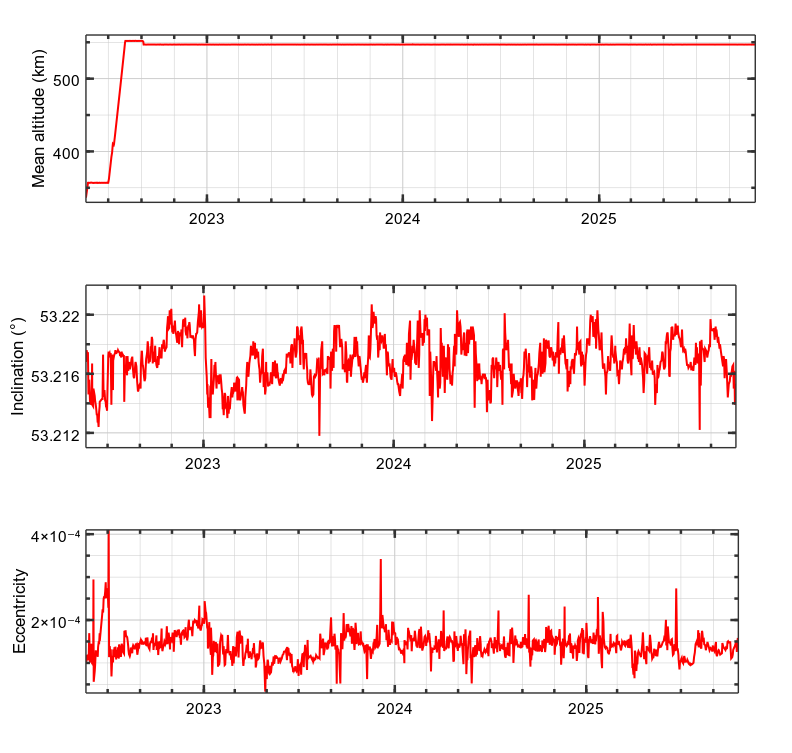
\includegraphics[width=\linewidth]{LaTeX/Figures/change_in_orbital_parameters.png}
    \caption{Plots of mean altitude, inclination and eccentricity for the entire mission duration of the \textit{Starlink-3988} satellite. Data taken from the In The Sky website~\cite{inthesky_starlink3988}.}
    \label{fig:parameters_plot_in_the_sky}
\end{figure}

Therefore, the constancy assumption on orbital parameters of eccentricity, semi-major axis and inclination carried throughout this report is demonstrated to be justified. Furthermore, as previously discussed in Section~\ref{sec:arg_of_perigee}, the argument of perigee carries no physical meaning due to the near-circular nature of the orbit, hence any discussion of its variation over time would be vacuous. The parameters left to discuss are then the true anomaly and right ascension of the ascending node (RAAN). True anomaly for a circular orbit has been demonstrated to be equivalent to mean anomaly, and its main usage is to identify the location of the satellite along the circular orbit at a given time. Its value consequently increases linearly over time, with a full revolution every orbital period. True anomaly has to be determined in a relative fashion, comparing it to a reference value (like we have done in the future prediction in Section~\ref{sec:mean_anomaly}). Any notion of the absolute value of mean anomaly is meaningless without an anchoring point. Hence, showing a plot of its evolution over time would not be very informative.

On the other hand, the most interesting parameter to discuss is RAAN. This is the parameter most affected by perturbations, namely, Earth’s oblateness. Due to the equatorial bulge, Earth’s gravitational field departs from perfect sphericity, introducing a second zonal harmonic (as well as other, less impactful, higher order variations), \( J_{2} \), in its gravitational potential. This asymmetry exerts a torque on the orbital plane, leading to a slow, secular precession of the node. The effect is strongest for low-altitude, inclined orbits, where the gravitational gradient across the orbit is more pronounced. For near-circular orbits such as ours, this precession does not change the shape or size of the orbit, but only rotates the orbital plane around the Earth’s axis. The direction of this precession depends on inclination: for prograde orbits such as ours (inclination \( i = 53.2^{\circ} < 90^{\circ} \)), the node is expected to regress (moves westward). The approximate rate of change can be expressed as (see lecture notes for derivation):
\[
\dot{\Omega} \approx -\frac{3}{2}J_{2}\left(\frac{R_{E}}{a}\right)^{2}n\cos i,
\]  
showing explicitly the dependence on the Earth’s equatorial radius \( R_{E} \), mean motion \( n \), semi-major axis \( a \), and inclination \( i \). For the analysed orbit with estimated \( \bar{a} = 6938~\text{km} \) and \( \bar{i} = 52.82^{\circ} \) (other values from Table~\ref{tab:starlink3988_orbit}, noting $J_2 = \num{1.08263e-3}$, dimensionless), this corresponds to a precession of approximately $-3.7$ degrees per day, or nearly two full $-360^{\circ}$ cycles every six months (3.8 a year).

\begin{figure}[h]
    \centering
    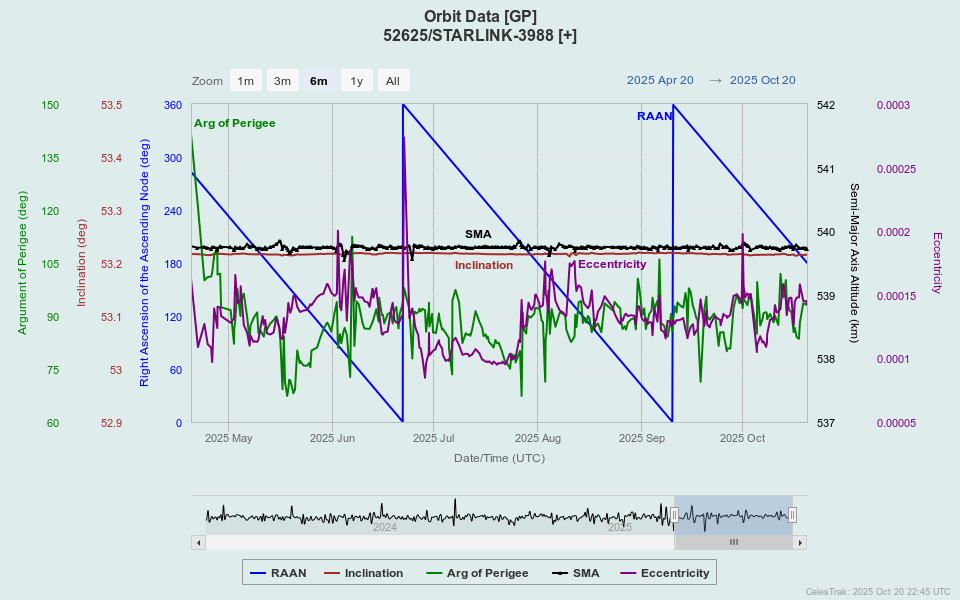
\includegraphics[width=\linewidth]{LaTeX/Figures/Orbit-Data-Starlink-3988.png}
    \caption{Plot of all six orbital parameters for six months prior to and including October 20th, 2025. Data from the Celestrak website~\cite{CelesTrak}.}
    \label{fig:parameters_plot_celestrak}
\end{figure}

This theoretical expectation is clearly confirmed by Figure~\ref{fig:parameters_plot_celestrak}, which displays the temporal evolution of the orbital parameters obtained from the CelesTrak database over six months. The top panel of the figure shows a gradual, monotonic regression in RAAN of about two cycles (over the six months), fully consistent with the expected nodal regression calculated above. Meanwhile, the figure also confirms that the remaining parameters (semi-major axis, inclination, and eccentricity), remain effectively constant within the noise of the dataset over the six-month period. This confirms that the only long-term variation of importance for our nearly circular orbit arises from the precession of the node caused by Earth’s oblateness, as predicted by perturbation theory discussed in recent lectures.

\section{Error Analysis} \label{sec:error_analysis}

A summary of the six orbital parameters estimated in this report, compared against reference TLE data, is provided in Table~\ref{tab:error_table}. For each element, the first column reports the true value from Table~\ref{tab:starlink3988_orbit}, the second shows our empirical estimate, and the third presents the relative percentage error.

\begin{table}[H]
    \centering
    \caption{Comparison between empirically estimated and TLE orbital parameters for \textit{Starlink-3988}.}
    \label{tab:error_table}
    \renewcommand{\arraystretch}{1.2}
    \begin{tabular}{|l|m{1.5cm}|m{2cm}|m{1cm}|m{3.5cm}|}
        \hline
        \textbf{Orbital Parameter} & \textbf{TLE Value} & \textbf{Estimated Value} & \textbf{Error (\%)} & \textbf{Comment} \\ \hline
        Semi-Major Axis, $a$ (\si{\kilo\metre}) & 6917 & 6938 & 0.30 & Highly reliable; direct result from accurate $\tau$ estimate. \\ \hline
        Eccentricity, $e$ () & 0.0001133 & 0.0148 $\pm$ 0.0194 & high & Unreliable; experimental precision insufficient to resolve such small values. \\ \hline
        Inclination, $i$ (\si{\degree}) & 53.2146 & 52.82 $\pm$ 0.44 & 0.73 & Reliable; within uncertainty range of TLE. \\ \hline
        RAAN, $\Omega$ (\si{\degree}) & 171.9324 & --- & N/A & Not measured; taken directly from TLE due to temporal limitation. \\ \hline
        Argument of Perigee, $\omega$ (\si{\degree}) & 95.0058 & --- & N/A & Undefined for near-circular orbits; physically meaningless here. \\ \hline
        True Anomaly, $\theta$ (\si{\degree}) & 265.1064 & 321.55 & 21.29 & Moderate; long propagation interval amplifies small period errors. \\ \hline
    \end{tabular}
\end{table}

 The most significant and reliable determination arises from the orbital period, which directly governs the semi-major axis through Kepler’s third law. Both parameters were measured with high consistency, yielding errors below one percent when compared with catalogue data. This accuracy can be attributed to the internal precision of Method~1, which averages multiple right ascension–declination pairs to suppress random noise and timing biases. Further, this is the task of the project towards which the most effort was invested, with detailed error and uncertainty analysis, including plots, refinements with outliar removal, and an extensive discussion, all present in Section~\ref{first_estimates_and_assumptions}.

By contrast, eccentricity proved intractable to estimate with the available data. The very small true value ($e \sim 10^{-4}$) is several orders of magnitude below the experimental sensitivity achievable through angular-velocity propagation, leading to a result dominated by numerical noise. Although our computed $e$ is formally nonzero, its associated uncertainty fully encompasses the true value, confirming that the orbit is effectively circular within measurement precision.

The inclination measurement demonstrates both consistency and practical reliability. The result agrees with the TLE value to within less than one degree, a deviation smaller than the propagated instrumental uncertainty from the azimuth–elevation data. This indicates that the geometric method used, though simplified, provides a credible estimate for $i$ when based on a clear mid-pass observation. However, it should be noted that the accuracy of the estimate was highly dependent on the selection of which data to adopt. We hypothesise that this is because observations taken near the mid-point of a pass sample the satellite when it is highest above the horizon and closest to the observer, which minimises projection errors.

For the argument of perigee and RAAN, no experimental determination was attempted. Both parameters are intrinsically difficult to measure over short observational windows: $\omega$ is undefined for circular orbits, while $\Omega$ varies only slowly over several days due to nodal precession and thus cannot be retrieved without long-term tracking. Their catalogue values are included purely for completeness. It should be noted that a lengthy discussion of the recession of RAAN was held in Section~\ref{sec:evolution_of_parameters}.

Finally, the propagation of mean anomaly over fifteen orbits yielded a phase difference of approximately $56.4^{\circ}$, corresponding to an error of $\sim21\%$. This relatively large discrepancy is physically interpretable: even a minute deviation in the measured orbital period accumulates over multiple revolutions, leading to significant phase drift. Our attempted prediction was ambitious at almost two days into the future, and a prediction over a smaller time window would likely have yielded better results. This highlights the sensitivity of mean and true anomaly predictions to small timing uncertainties and justifies why long-term propagation using observationally derived periods is inherently unstable.

Beyond these geometric considerations, several other sources of uncertainty were identified and quantified across different parts of this report. These include: (1) human reaction and timing errors during visual data collection (discussed in Section~\ref{sec:data}); (2) rounding and discretisation in the conversion from azimuth–elevation to right ascension–declination coordinates; (3) limited temporal resolution in online tracking datasets, particularly in Method~4; (4) the simplifying assumption of circular motion, which introduces small systematic biases when eccentricity is non-zero; and (5) atmospheric and refraction effects near the horizon, which become significant during low-elevation measurements. The propagation of these uncertainties was explicitly derived for the period, angular velocity, and eccentricity estimates in Sections~\ref{first_estimates_and_assumptions} and~\ref{sec:eccentricity}. Collectively, these constitute the dominant contributions to the experimental error budget and justify the relative weighting of confidence assigned to each parameter. Several improvements could be implemented to reduce these errors in future experiments. First, an automated timestamping system or digital photometric tracker would remove human latency in manual time logging (although this was already implemented for Method 4, later discarded). Second, recording data at multiple ground stations or over consecutive nights would allow RAAN and nodal precession to be empirically measured rather than inferred from TLEs. Third, acquiring higher-frequency angular data (for instance, one sample per second rather than per minute) would improve the fidelity of $\omega$ and $\theta$ propagation, with the caveat of increasing data-processing demands. Finally, applying a least-squares orbital fit to multiple passes, rather than using discrete pairwise comparisons, would reduce random scatter and provide statistically rigorous uncertainties when estimating the orbital period. These methodological refinements would strengthen the precision of future empirical orbital determinations while maintaining the accessible, ground-based approach of this project.

Overall, the experiment achieved acceptable agreement for geometric and temporal parameters (semi-major axis, inclination, and period), while anomalies and shape descriptors (eccentricity and true anomaly) remain constrained by measurement limits and simplifying assumptions. These outcomes confirm that, despite the modest tools used, the circular-orbit approximation and two-body framework adopted throughout the report provide a valid and self-consistent characterisation of the \textit{Starlink-3988} orbit.

\section{Conclusion}

This project has demonstrated the practical determination of a satellite’s orbit through a combination of observational data and theoretical orbital mechanics. Using a series of elevation and azimuth measurements recorded across multiple passes of \textit{Starlink-3988}, each of the six classical orbital parameters was derived and compared against official Two-Line Element (TLE) values. The methods employed showed encouraging consistency, particularly for orbital period, semi-major axis and inclination, which matched the published data within the propagated measurement uncertainty. 

Beyond the numerical results, the project offered a clear understanding of how theoretical models connect with real-world observation. Through this process, I personally developed a great appreciation for how orbital mechanics, while elegantly simple in formulation, demands careful treatment of data and assumptions to yield meaningful predictions. On top of this, I have strengthened my admiration for Starlink and its constellation: by continuously tracking satellites in the night sky, I quickly realised just how many Starlink units are present in the heavens, and constantly zooming by as we live our lives in negligence of this engineering marvel. Finally, the experience of observing, processing, and critically comparing results created a stronger physical intuition for orbital motion and an appreciation and admiration for the challenges faced by mission analysts who perform these calculations at professional accuracy.



\section{Visualisation}
\begin{center}
    \textit{Although specifically required by the project instructions, we noticed the mark scheme included no points for the visualisation step. It was assumed that this was once again an artefact of a year-over-year revision. We nevertheless exhausted this step for completeness.}
\end{center}

A visualisation of the results reported in Table~\ref{tab:error_table} is displayed in Figure~\ref{fig:data_visualisation}, which compares the estimated parameters with the TLE data. The most noticeable difference in the two orbits is the error in true (mean) anomaly, as the two satellites appear at different locations along their orbits. The plots were created using \texttt{Python}, and the code developed to create them is also available at the supporting repository.

\begin{figure}
    \centering
    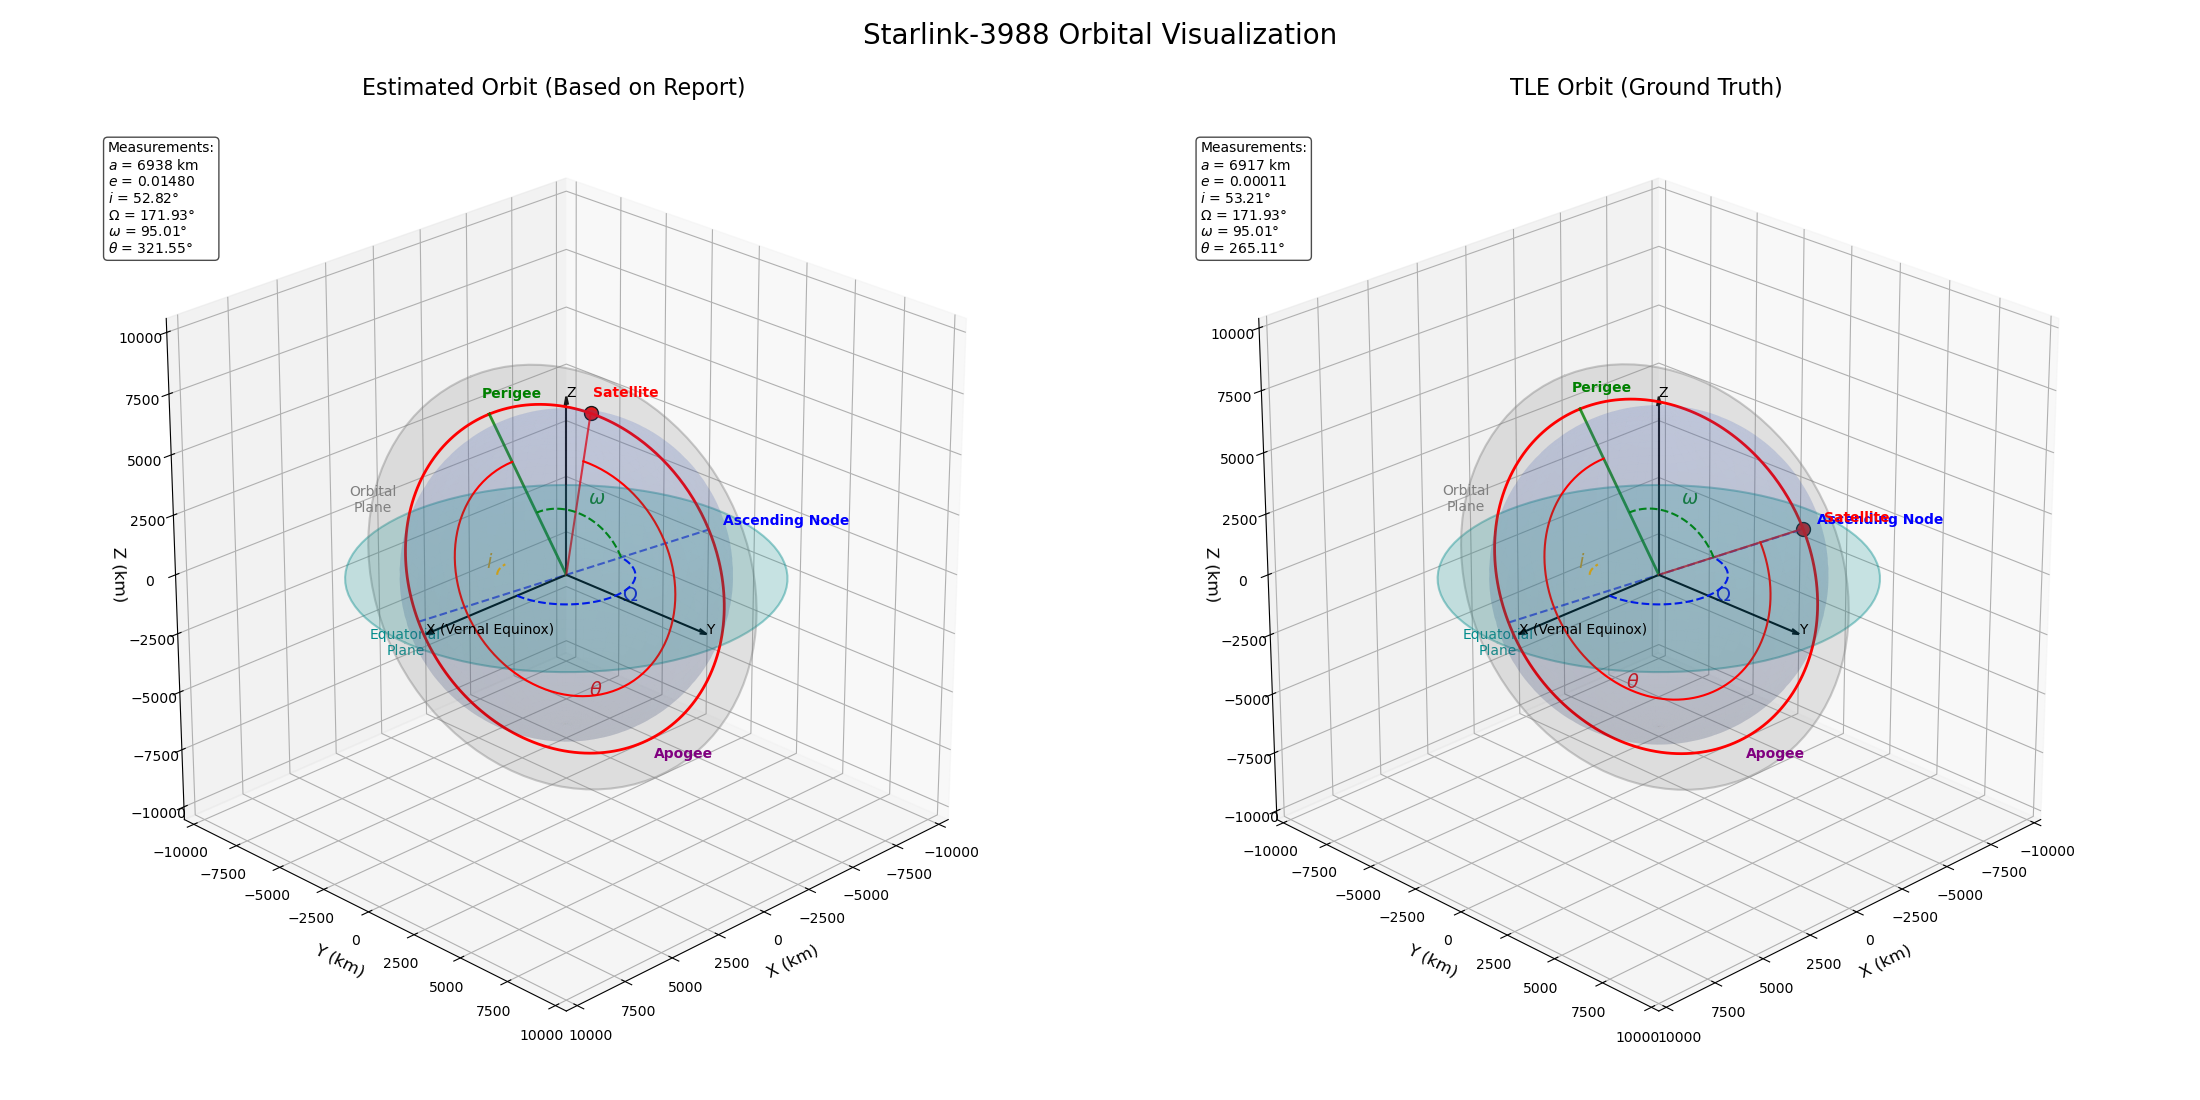
\includegraphics[width=\linewidth]{LaTeX/Figures/Orbital_Plots.png}
    \caption{A visualisation of the estimated and TLE orbital data. The left figure shows the estimated data, the right figure the TLE data.}
    \label{fig:data_visualisation}
\end{figure}

\printbibliography

\newpage
\appendix
\section{Appendix} \label{Appendix}

Screenshots of the mobile apps used for the observations. The screenshots show the last observation taken on 10/20, and are labelled to distinguish them from other similar screenshots. Figure~\ref{fig:tracker_screenshot} shows the Satellite Tracker mobile app in use on a Samsung Galaxy S24 Ultra. Figure~\ref{fig:tracker_pro_screenshot} shows the Satellite Tracker Pro app in use on an iPhone 12.

\begin{figure}[h!]
    \centering

    \begin{subfigure}[b]{0.35\textwidth}
        \centering
        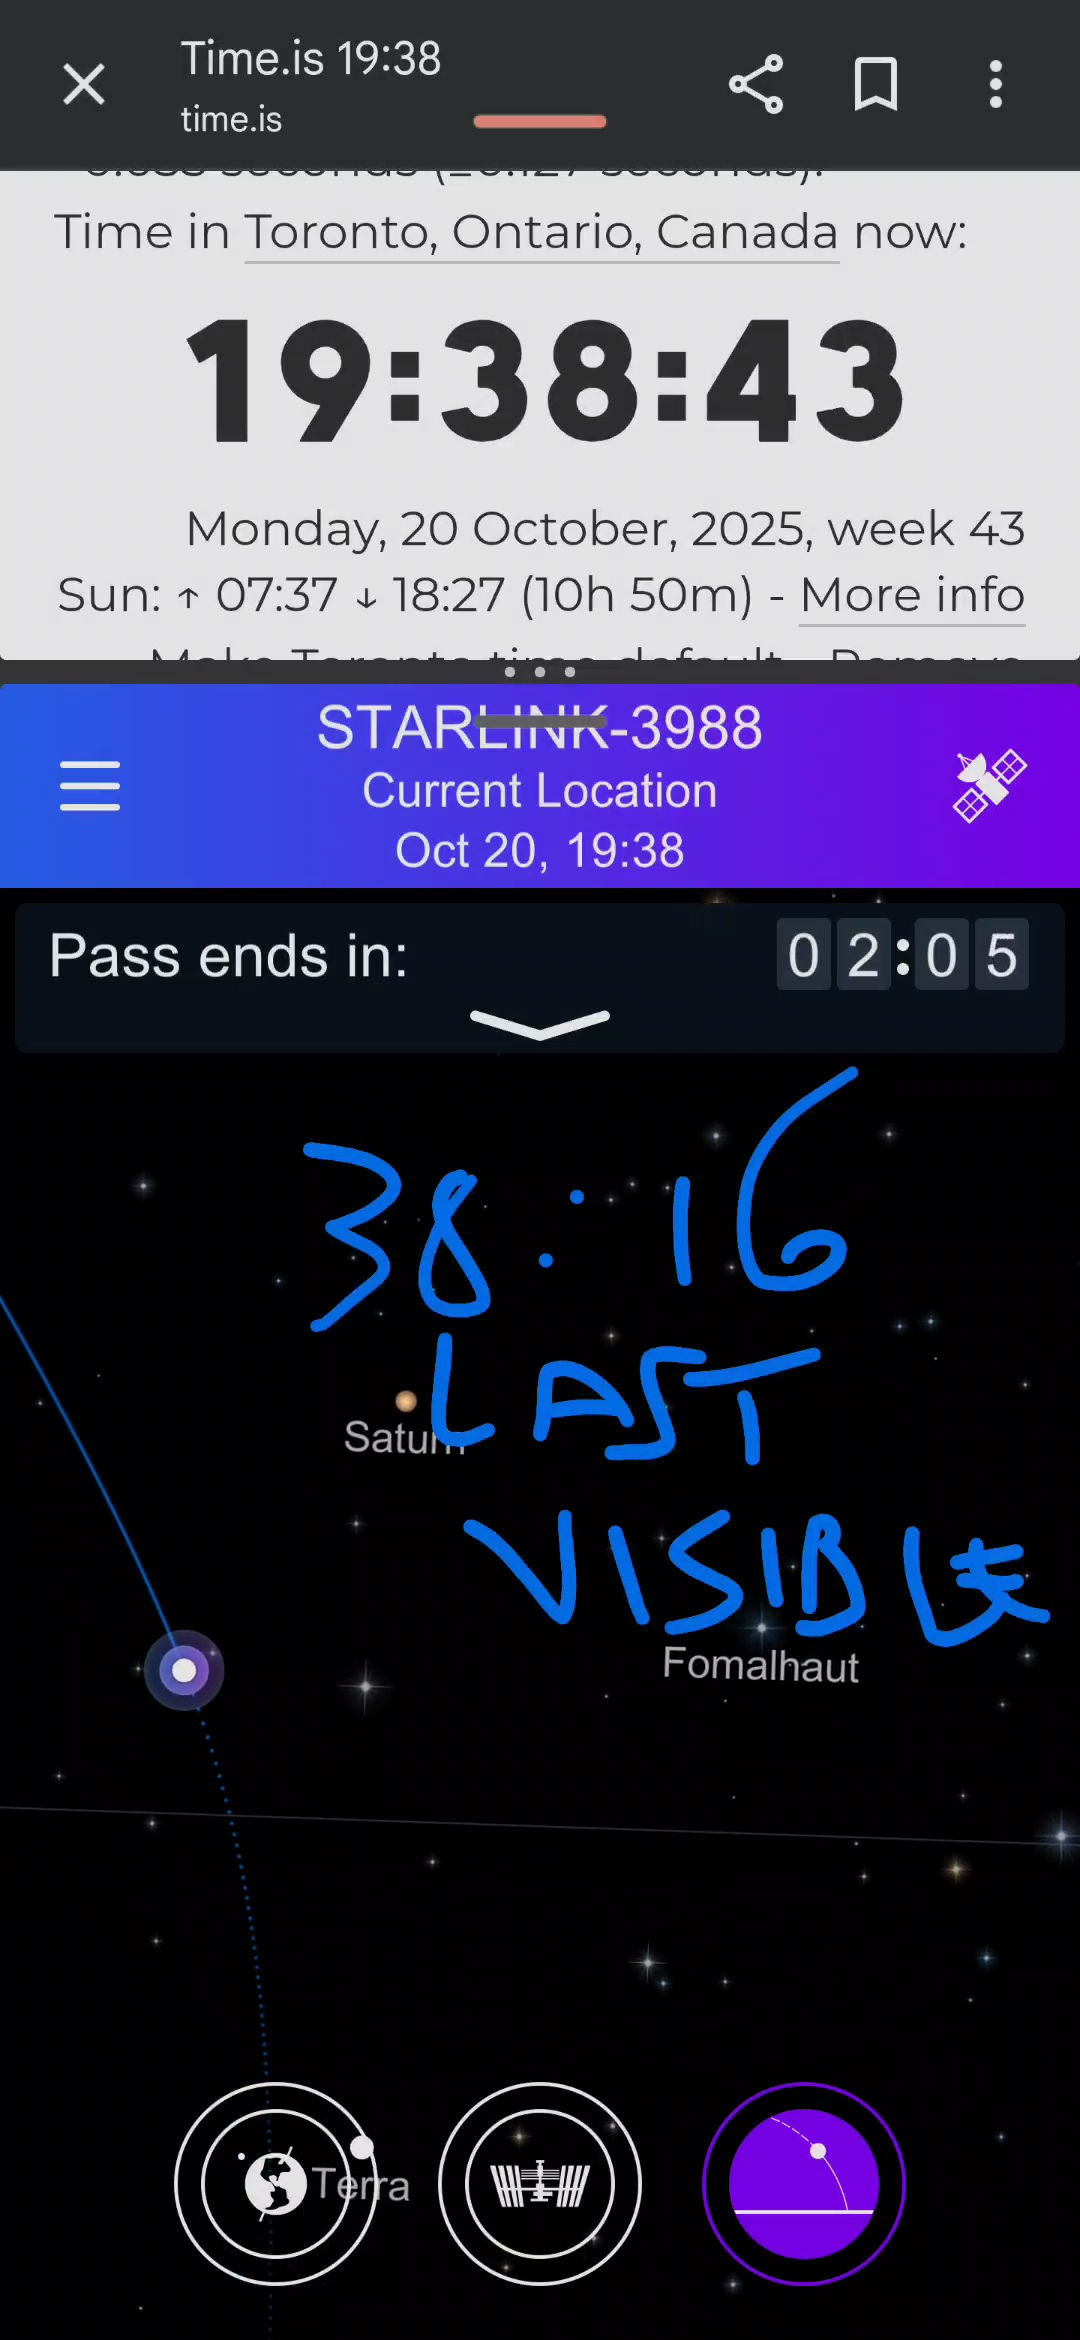
\includegraphics[width=\textwidth]{LaTeX/Figures/Satellite_Tracker_Screenshot.jpg}
        \caption{Satellite Tracker app.}
        \label{fig:tracker_screenshot}
    \end{subfigure}
    \begin{subfigure}[b]{0.35\textwidth}
        \centering
        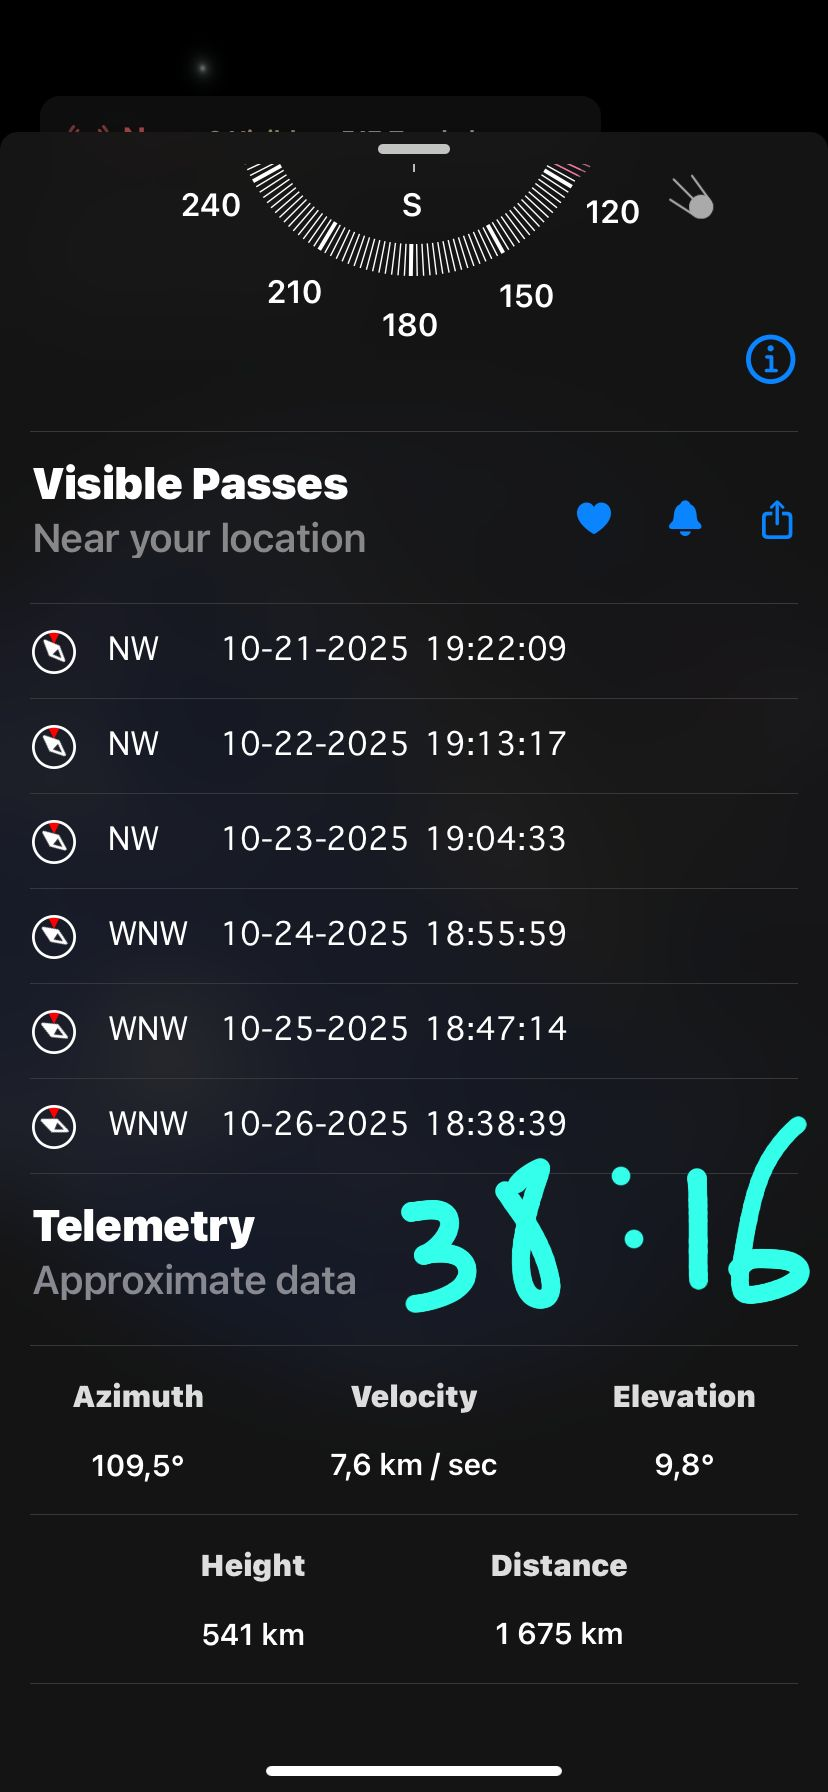
\includegraphics[width=\textwidth]{LaTeX/Figures/Satellite_Tracker_Pro_Screenshot.jpg}
        \caption{Satellite Tracker Pro app.}
        \label{fig:tracker_pro_screenshot}
    \end{subfigure}
    
\end{figure}

Table~\ref{tab:method1_data_comparison} shows the data collected from the In The Sky website in preparation for the measurement later carried out with mobile apps for Method 1.

\begin{table}[H]
    \centering
    \caption{Comparison data from the In The Sky website.}
    \label{tab:method1_data_comparison}
    \renewcommand{\arraystretch}{1.2}
    \begin{tabular}{|c|c|c|c|c|c|}
        \hline
        \textbf{Date} & \textbf{Time} & \textbf{Azimuth} & \textbf{Elevation} & \textbf{Right} & \textbf{Declination} \\ 
        \textbf{ } & \textbf{ } & \textbf{(°)} & \textbf{Angle (°)} & \textbf{Ascension (°)} & \textbf{(°)} \\ \hline
        \multicolumn{6}{|c|}{\textbf{Observation 1}} \\ \hline
        10/19 & 19:39:15 & 321.0 & 10.0 & 189.3 & 43.8 \\ \hline
        10/19 & 19:40:00 & 324.5 & 13.9 & 189.5 & 49.3 \\ \hline
        10/19 & 19:41:00 & 333.4 & 21.7 & 188.3 & 60.8 \\ \hline
        10/19 & 19:42:00 & 350.5 & 32.1 & 175.8 & 78.7 \\ \hline
        10/19 & 19:43:00 & 024.8 & 41.0 & 029.8 & 71.3 \\ \hline
        10/19 & 19:44:00 & 061.3 & 37.0 & 023.0 & 43.0 \\ \hline
        10/19 & 19:45:00 & 084.6 & 26.1 & 022.3 & 20.4 \\ \hline
        10/19 & 19:46:00 & 096.2 & 16.9 & 022.8 & 06.3 \\ \hline
        10/19 & 19:46:29 & 102.5 & 10.2 & 023.8 & -03.7 \\ \hline
    \end{tabular}
\end{table}

\newpage
Figure~\ref{fig:n2yo_screenshot} shows a screenshot of a frame from the screen recording of the N2YO website used for Method 4. The screen recording was carried out over several hours on a Windows 11 Razer Blade 14 using the Snipping Tool app.

\begin{figure}[h]
    \centering
    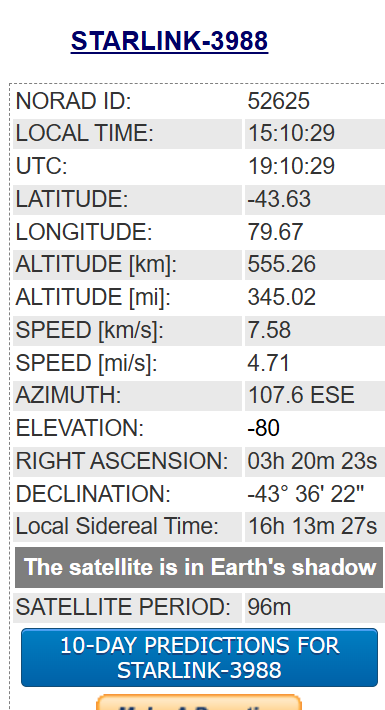
\includegraphics[width=0.5\linewidth]{LaTeX/Figures/N2YO .png}
    \caption{A frame from the screen recording of the N2YO website.}
    \label{fig:n2yo_screenshot}
\end{figure}

\newpage
\section*{Appendix B: Reading a Two-Line Element Set (TLE)}
\label{AppendixB}

Two-Line Element (TLE) sets provide the standard format used by NORAD and NASA to describe the orbital parameters of Earth-orbiting satellites. Each TLE consists of two lines of numerical data that together define the satellite's orbit at a given epoch. The TLE format is used by most satellite-tracking software and online resources, including N2YO~\cite{n2yo_starlink3988}, and is compatible with propagation models such as SGP4.

\noindent The following TLE corresponds to \textit{Starlink-3988}, obtained from N2YO on 21~October~2025:

\begin{verbatim}
1 52625U 22052AD  25294.95368970  .00001040  00000-0  83377-4 0  9997
2 52625  53.2146 171.9324 0001133  95.0058 265.1064 15.08848508190040
\end{verbatim}

\subsection*{Line 1: Identification and Timing Information}

\begin{itemize}
    \item Column 1: Line number (always 1 for the first line of the TLE).
    \item Columns 3 - 7: Satellite catalogue number. Here \texttt{52625} is the unique NORAD identification number assigned to \textit{Starlink-3988}.
    \item Column 8: Classification. The letter \texttt{U} indicates that the satellite is unclassified.
    \item Columns 10 - 17: International designator. The entry \texttt{22052AD} specifies the launch year (2022), the launch number (52), and the sequential piece identifier (AD).
    \item Columns 19 - 32: Epoch time. The value \texttt{25294.95368970} represents the year 2025 and the fractional day 294.95368970, corresponding to 21~October~2025 at 22:53:19~UTC (18:53:19 EDT). The epoch indicates the instant at which all the orbital parameters are valid.
    \item Columns 34--43: First time derivative of mean motion. The value \texttt{.00001040} represents the rate of change in the mean motion (revolutions per day) due to atmospheric drag.
    \item Columns 45 - 52: Second derivative of mean motion. The value \texttt{00000-0} is typically zero, as higher-order drag effects are negligible.
    \item Columns 54 - 61: BSTAR drag term. The value \texttt{83377-4} corresponds to a drag coefficient of \(8.3377\times10^{-4}\) (in reciprocal Earth radii). This parameter quantifies the effect of atmospheric drag on the satellite’s motion.
    \item Column 63: Ephemeris type. A value of \texttt{0} indicates use of the standard SGP4 orbital model.
    \item Columns 65 - 68: Element set number. The entry \texttt{999} identifies the current version of the orbital element set.
    \item Column 69: Checksum. The digit \texttt{7} ensures the integrity of the data line.
\end{itemize}

\subsection*{Line 2: Orbital Elements}

\begin{itemize}
    \item Column 1: Line number (always 2 for the second line of the TLE).
    \item Columns 3 - 7: Satellite number. The entry \texttt{52625} matches the value in Line~1.
    \item Columns 9 - 16: Inclination. The value \texttt{53.2146\si{\degree}} gives the angle between the orbital plane and the Earth's equatorial plane.
    \item Columns 18 - 25: Right Ascension of the Ascending Node (RAAN). The value \texttt{171.9324\si{\degree}} specifies the longitude where the satellite crosses the equator from south to north.
    \item Columns 27 - 33: Eccentricity. The digits \texttt{0001133} imply \(e = 0.0001133\). The decimal point is omitted in the TLE format but is understood to lie immediately before the first digit.
    \item Columns 35 - 42: Argument of Perigee. The value \texttt{95.0058\si{\degree}} is the angle, measured in the orbital plane, from the ascending node to the perigee.
    \item Columns 44 - 51: Mean Anomaly. The value \texttt{265.1064\si{\degree}} specifies the satellite’s position in its orbit at the epoch time.
    \item Columns 53 - 63: Mean Motion. The value \texttt{15.08848508} represents the number of orbital revolutions completed per sidereal day.
    \item Columns 64 - 68: Revolution number at epoch. The entry \texttt{19004} is the total number of orbits completed since launch.
    \item Column 69: Checksum. The digit \texttt{0} provides a line integrity check for the second line.
\end{itemize}

\subsection*{Derived Orbital Parameters}

From the mean motion \(n = 15.08848508~\si{rev/day}\), the orbital period is obtained as:
\[
\tau = \frac{1440}{n} = \SI{95.43}{\minute}.
\]
Using Kepler’s third law, the corresponding semi-major axis is determined as:
\[
a = \left(\frac{\mu}{(2\pi n / 86400)^{2}}\right)^{1/3} \approx \SI{6917}{\kilo\metre}.
\]
The eccentricity, inclination, and other parameters further allow for a calculation of the perigee and apogee altitudes:  the perigee and apogee distances (measured from the Earth's centre) are first obtained from the semi-major axis \(a\) and the orbital eccentricity \(e\) as:
\[
r_{p} = a(1 - e),
\qquad
r_{a} = a(1 + e).
\]
The corresponding altitudes above the Earth's surface are then:
\[
h_{p} = r_{p} - R_{E},
\qquad
h_{a} = r_{a} - R_{E},
\]
where \(R_{E}\) is the mean radius of the Earth. The mean orbital altitude \(h\) is the arithmetic mean of the perigee and apogee altitudes:
\[
h = \frac{h_{p} + h_{a}}{2}
    = \frac{(r_{p} - R_{E}) + (r_{a} - R_{E})}{2}
    = a - R_{E}.
\]
Hence, for nearly circular orbits (\(e \approx 0\)), the mean altitude simplifies to the difference between the semi-major axis and the Earth's mean radius. These TLEs were used to produce the orbital parameters summarised in Table~\ref{tab:starlink3988_orbit}.

\end{document}
